%% ------------------------------------------------------------------- %%
%% ------------------------------------------------------------------- %%
%% ------------------------------------------------------------------- %%
%% ------------------------------------------------------------------- %%
\chapter{Experimentos y Resultados}
\label{cap:resultados}

\lhead{\emph{Experimentos y Resultados}} 

%% ------------------------------------------------------------------- %%
%% ------------------------------------------------------------------- %%
%% ------------------------------------------------------------------- %%
%% ------------------------------------------------------------------- %%
%% ------------------------------------------------------------------- %%
%% ------------------------------------------------------------------- %%

%% -------------------------------------------------------------------- %%
%% -------------------------------------------------------------------- %%

En este capítulo, detallamos los resultados del \textit{fine-tuning} de los modelos \textit{Transformers} y el efecto de aplicar \textit{Gradient Accumulation Steps} (GAS)  y una metodología de congelación de capas. Al principio, entrenamos cada modelo durante tres \textit{epochs}; luego, seleccionamos los modelos con los mejores resultados y los entrenamos nuevamente durante 30 \textit{epochs} con \textit{early stopping}.

\section{Congelación de Capas}

Para la metodología de congelación de capas, congelamos todos los parámetros del \textit{Transformer} y solo entrenamos el bloque BiLSTM. Utilizar este método acelera el entrenamiento y mantiene el buen rendimiento, como se ha discutido en trabajos previos \citep{merchant2020happens,lee2019would,kovaleva2019revealing}.

La comparación de desepeño se presenta en la Tabla \ref{tab:comparison_3_epochs}; además, la Figura \ref{fig:comparison_3_3pochs}(a) muestra el AUC de cada modelo utilizando GAS y la metodología de congelación de capas. En esta comparación, el sufijo 'Normal' representa el entrenamiento  utilizando todos los hiperparámetros de la Sección \ref{sec:fine-tuned}; el sufijo 'GAS' indica la integración de \textit{Gradient Accumulation Steps} (GAS), mientras que el sufijo 'Freeze' indica la aplicación de la metodología de congelación de capas a los modelos. Según los resultados obtenidos, es evidente que la implementación de la metodología de congelación de capas conduce a mejoras en el rendimiento en todos los modelos ESM2. Además, se observó que los modelos más grandes, como ESM2(t30)-Normal, ESM2(t33)-Normal, TAPE-Normal y ProtBert-Normal, no lograron converger debido a un problema de \textit{vanish gradients}, lo cual se desarrollará en la sección posterior. Además, la utilización de la metodología de congelación de capas permite que estos modelos converjan de manera efectiva.

\begin{table}[h]
	\centering
	\caption[Comparación de los modelos \textit{Transformer} entrenados por 3 \textit{epochs}.]{Evaluación del rendimiento de los modelos de \textit{Transformer} utilizando \textit{Gradient Accumulation Steps} (GAS) y la metodología de congelación de capas, \textbf{entrenados durante tres \textit{epochs}}. Además, el sufijo 'Normal' representa el entrenamiento clásico utilizando los hiperparámetros de la Sección \ref{sec:fine-tuned}. La inclusión del sufijo 'GAS' en cada modelo indica la integración de \textit{Gradient Accumulation Steps}, mientras que el sufijo 'Freeze' señala la aplicación de la metodología de congelación de capas a los modelos. Además, el guion '-' en cada celda indica que el modelo no logro converger.}
	\label{tab:comparison_3_epochs}
	
	\scriptsize
	\setlength{\tabcolsep}{0.5em} % for the horizontal padding
	{\renewcommand{\arraystretch}{1.5}% for the vertical padding
	\begin{tabular}{lllllll} 
		\textbf{Modelo}       & \textbf{Accuracy} & \textbf{Precision} & \textbf{Recall} & \textbf{F1-score} & \textbf{AUC}    & \textbf{MCC}    \\ \midrule
		ESM2(t6)-Normal             & 0.9344            & \textbf{0.9334}    & 0.9354          & 0.9344            & 0.9805          & 0.8689          \\
		ESM2(t6)-Freeze      & \textbf{0.9351}   & 0.9253             & \textbf{0.9464} & \textbf{0.9357}   & \textbf{0.9812} & \textbf{0.8704} \\
		ESM2(t6)-GAS         & 0.8986            & 0.8966             & 0.9007          & 0.8986            & 0.9602          & 0.7973          \\
		ESM2(t6)-Freeze-GAS  & 0.8869            & 0.8913             & 0.8806          & 0.8860            & 0.9520          & 0.7738          \\ \midrule
		ESM2(t12)-Normal            & 0.9327            & 0.9243             & 0.9422          & 0.9332            & 0.9799          & 0.8655          \\
		ESM2(t12)-Freeze     & \textbf{0.9344}   & \textbf{0.9251}    & \textbf{0.9451} & \textbf{0.9350}   & \textbf{0.9808} & \textbf{0.8690} \\
		ESM2(t12)-GAS        & 0.9010            & 0.9279             & 0.8692          & 0.8976            & 0.9655          & 0.8037          \\
		ESM2(t12)-Freeze-GAS & 0.8805            & 0.8556             & 0.9149          & 0.8843            & 0.9475          & 0.7629          \\ \midrule
		ESM2(t30)-Normal            & -                 & -                  & -               & -                 & -               & -               \\
		ESM2(t30)-Freeze     & \textbf{0.9303}   & \textbf{0.9185}    & \textbf{0.9440} & \textbf{0.9311}   & \textbf{0.9786} & \textbf{0.8609} \\
		ESM2(t30)-GAS        & 0.9090            & 0.9167             & 0.8993          & 0.9079            & 0.9675          & 0.8181          \\
		ESM2(t30)-Freeze-GAS & 0.8565            & 0.8156             & 0.9206          & 0.8649            & 0.9312          & 0.7191          \\ \midrule
		ESM2(t33)-Normal            & -                 & -                  & -               & -                 & -               & -               \\
		ESM2(t33)-Freeze     & \textbf{0.6818}   & \textbf{0.7139}    & 0.6044          & 0.6546            & \textbf{0.7613} & 0.3677          \\
		ESM2(t33)-GAS        & 0.6767            & 0.6312             & 0.8467          & 0.7233            & 0.7442          & \textbf{0.3763} \\
		ESM2(t33)-Freeze-GAS & 0.6738            & 0.6254             & \textbf{0.8633} & \textbf{0.7254}   & 0.7514          & 0.3763          \\ \midrule
		TAPE-Normal                 & -                 & -                  & -               & -                 & -               & -               \\
		TAPE-Freeze          & 0.9342            & 0.9276             & 0.9415          & 0.9345            & 0.9809          & 0.8684          \\
		TAPE-GAS             & \textbf{0.9371}   & \textbf{0.9290}    & \textbf{0.9463} & \textbf{0.9376}   & \textbf{0.9826} & \textbf{0.8744} \\
		TAPE-Freeze-GAS      & 0.8914            & 0.8851             & 0.8989          & 0.8920            & 0.9564          & 0.7828          \\ \midrule
		ProtBert-Normal             & -                 & -                  & -               & -                 & -               & -               \\
		ProtBert-Freeze      & 0.9083            & 0.9176             & 0.8968          & 0.9071            & 0.9673          & 0.8168          \\
		ProtBert-GAS         & \textbf{0.9138}   & \textbf{0.9569}    & 0.8662          & \textbf{0.9093}   & \textbf{0.9767} & \textbf{0.8313} \\
		ProtBert-Freeze-GAS  & 0.7864            & 0.7333             & \textbf{0.8988} & 0.8076            & 0.8669          & 0.5881         \\ 
	\end{tabular}}
\end{table}

\clearpage

\begin{figure}[H]
	\centering
	\subfigure[Comparación por modelo.]{\label{fig:a}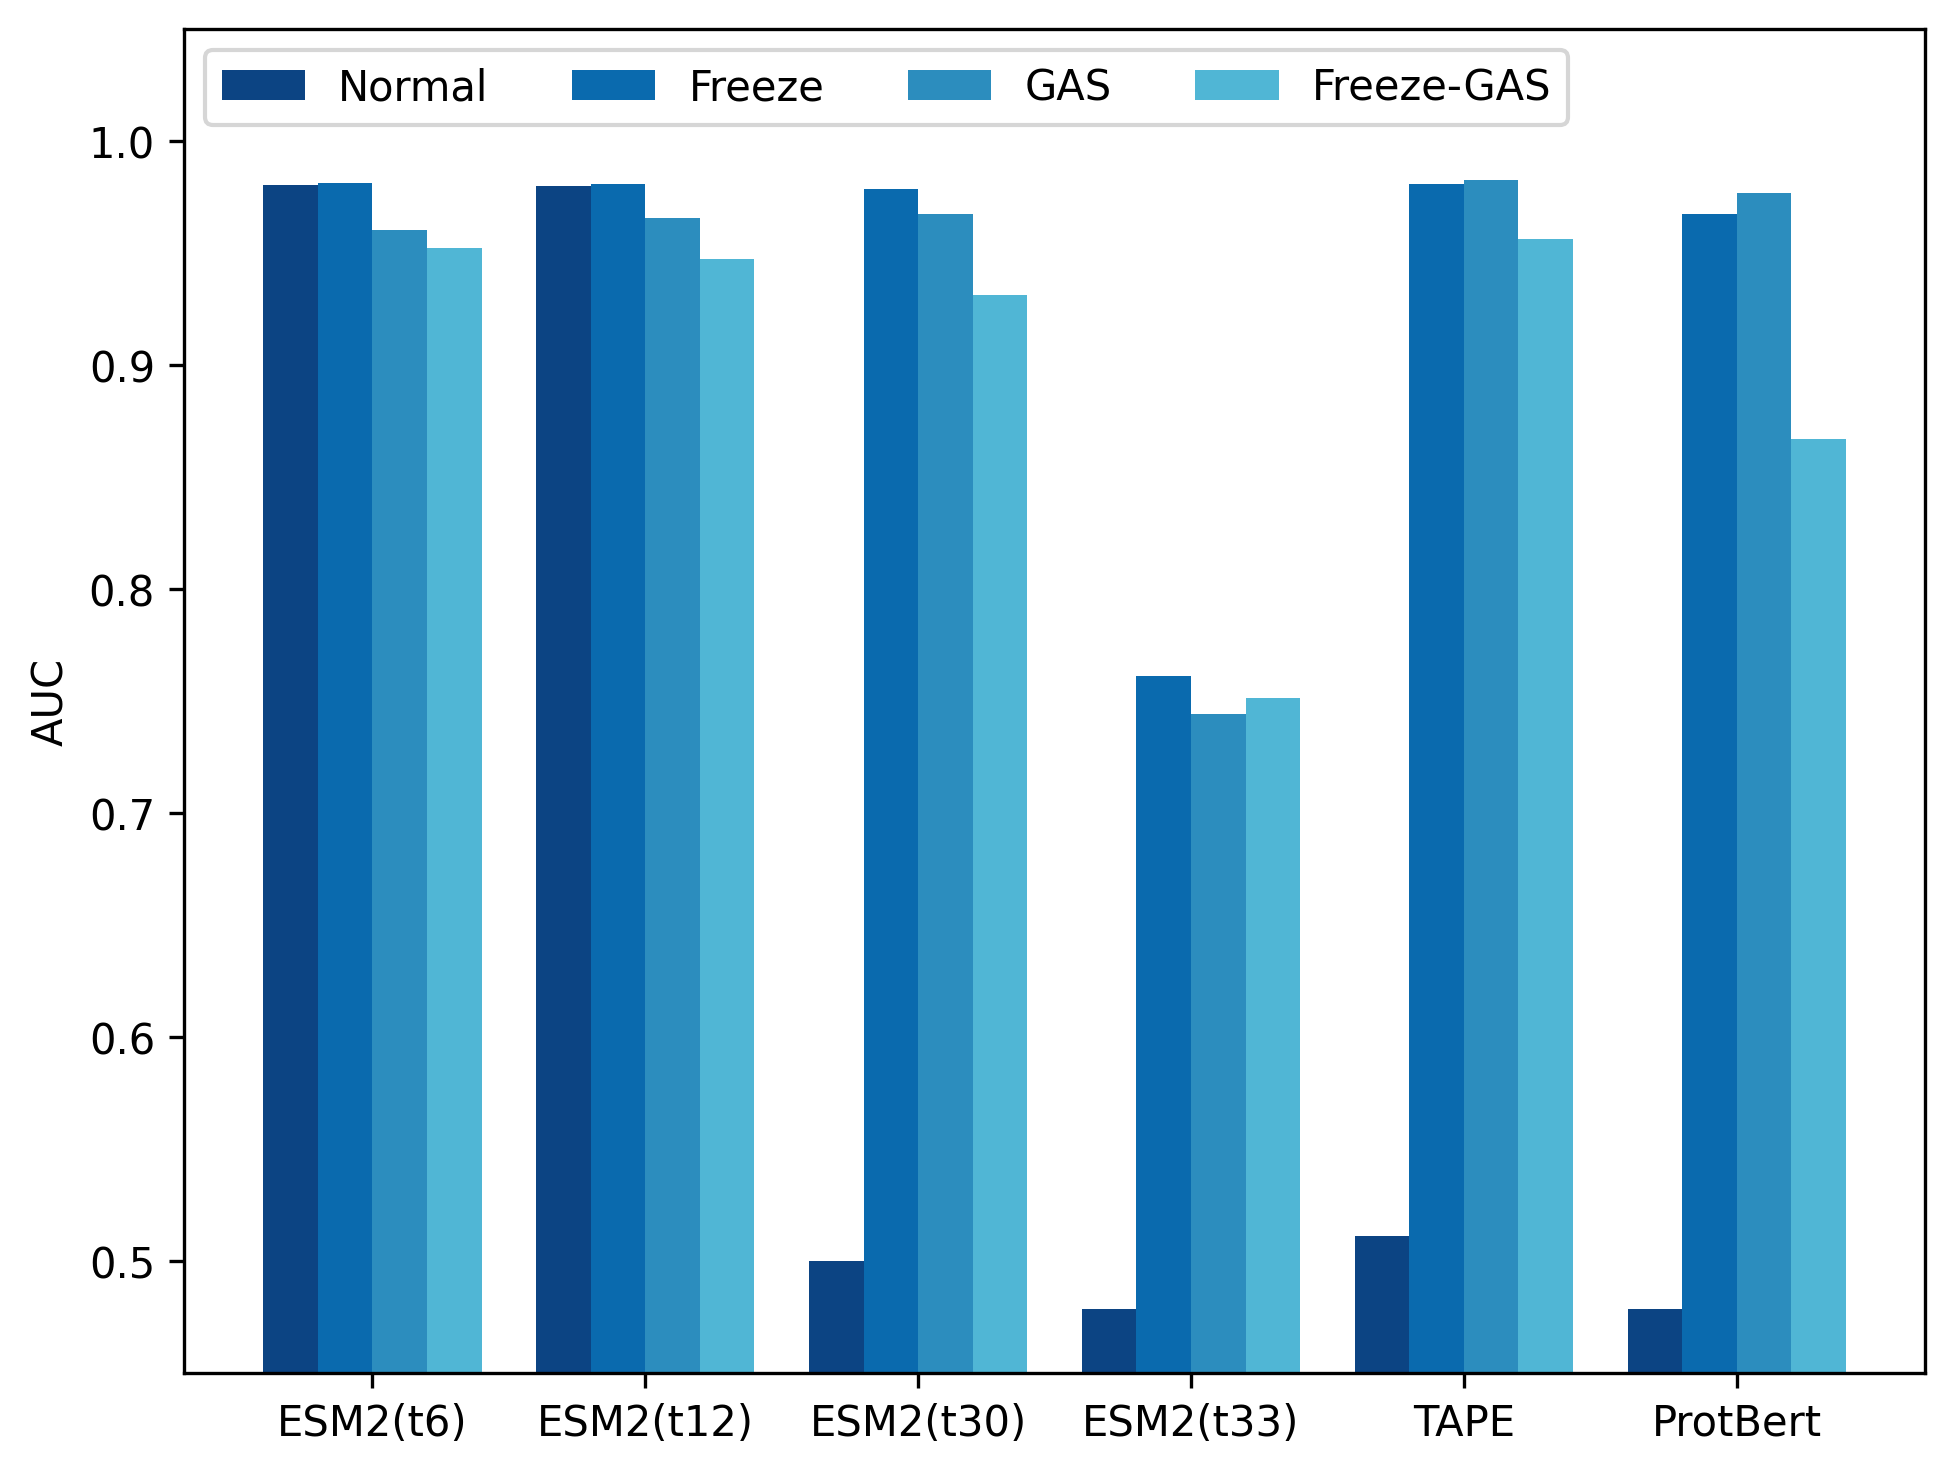
\includegraphics[width=0.8\textwidth]{img/results/metrics_comparion_by_model}}
	\subfigure[Comparación por la metodología de entrenamiento.]{\label{fig:b}	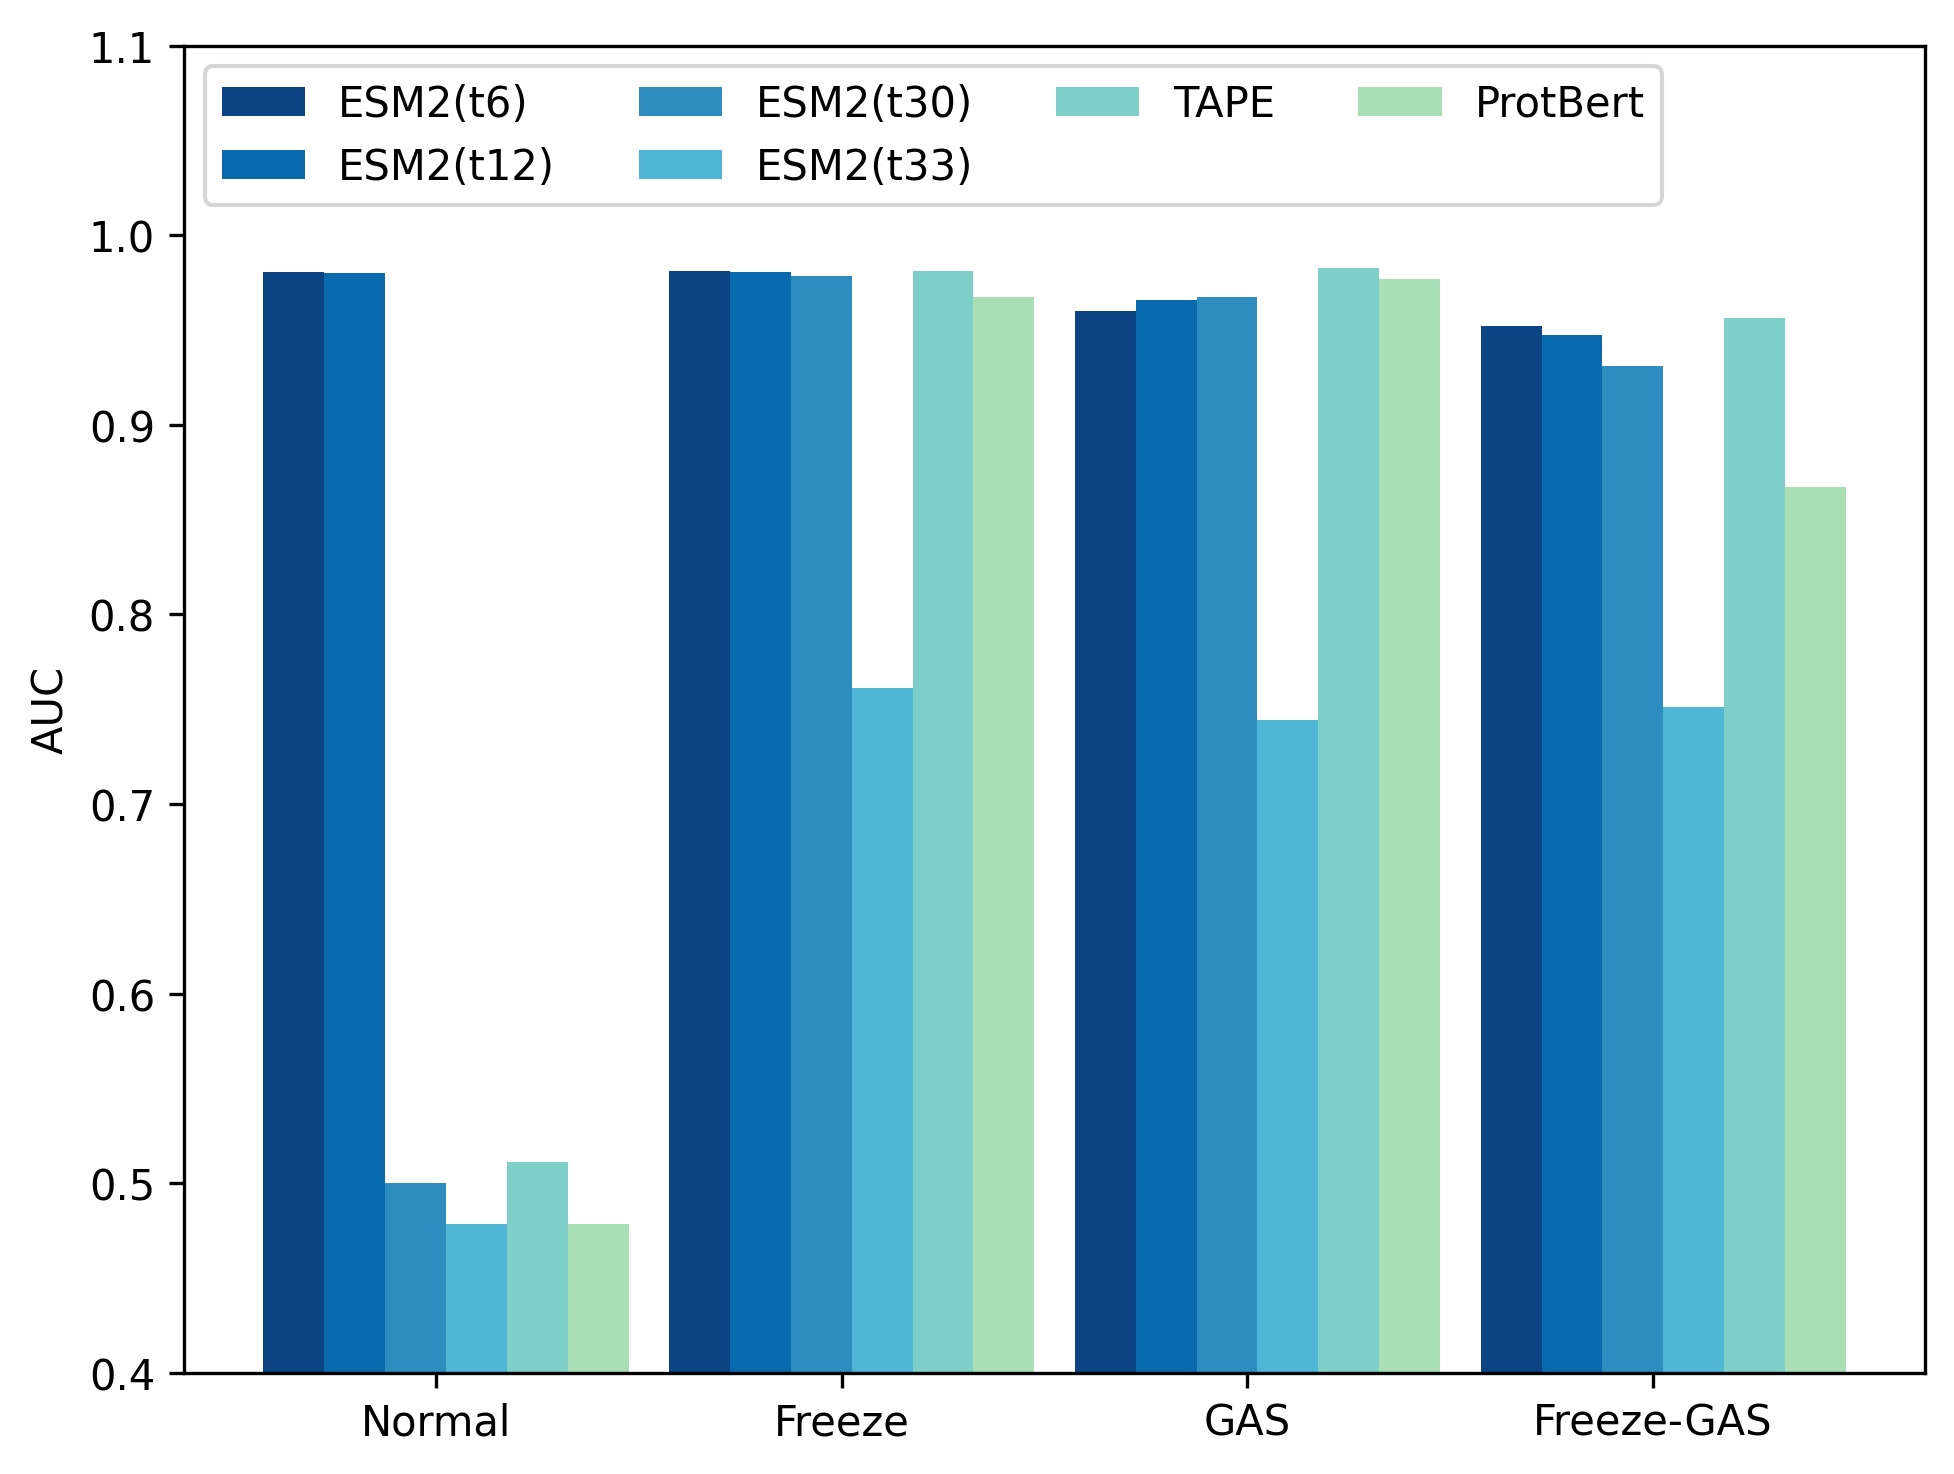
\includegraphics[width=0.8\textwidth]{img/results/metrics_comparion_by_type}}
	

	\caption[Comparación del AUC de modelos \textit{Transformers} entrenados con 3 \textit{epochs}]{Análisis comparativo de AUC en arquitecturas de modelos \textit{Transformers} utilizando diversas metodologías de entrenamiento, incluyendo el entrenamiento estándar (Normal), el entrenamiento con una metodología de congelación de capas (Freeze), el entrenamiento con \textit{Gradient Accumulation Steps} (GAS) y el entrenamiento combinando GAS con la congelación de capas (Freeze-GAS). Además, entrenamos todos los modelos durante tres \textit{epochs}.}
	\label{fig:comparison_3_3pochs}
\end{figure}

\section{\textit{Vanish Gradient} y GAS}

En la Tabla \ref{tab:comparison_3_epochs}, notamos que los modelos grandes como ESM2(t30)-Normal, ESM2(t33)-Normal, TAPE-Normal y ProtBert-Normal no lograron converger. Por lo tanto, graficamos los gradientes de estos modelos durante el entrenamiento para descubrir sus causas. En primer lugar, graficamos los gradientes promedio por capa para el modelo más pequeño, ESM2(t6)-Normal, en la Figura \ref{fig:t6} (este modelo no tuvo problemas de \textit{vanish gradient}). Luego, graficamos los gradientes promedio para ESM2(t30)-Normal (este modelo experimentó un problema de \textit{vanish gradient}) en la Figura \ref{fig:t30}. Como se desprende de los resultados, el modelo más grande, ESM2(t30), mostró gradientes promedio casi nulos en todas las capas de BERT después de solo tres épocas; como resultado, este fenómeno hizo que el modelo no logre converger de manera efectiva.

\begin{figure}[H]
	\centering
	\subfigure[Gráfico de los gradientes por capa antes de entrenar ESM2(t6).]{\label{fig:a}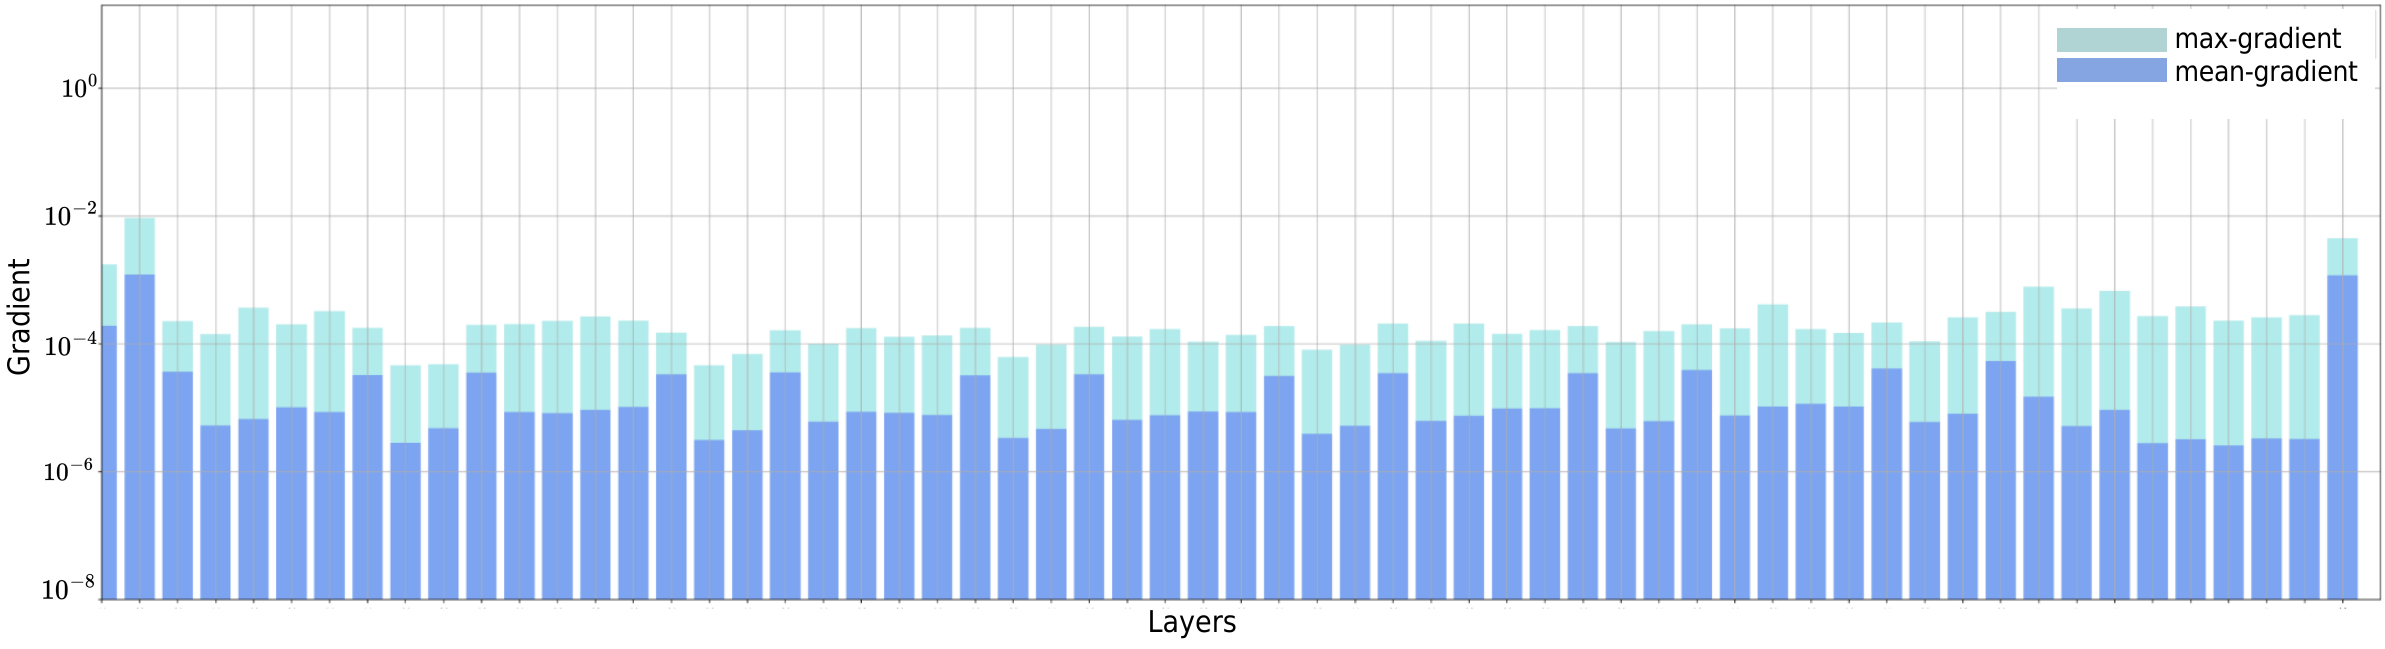
\includegraphics[width=\textwidth]{img/results/t6_epoch0}}
	\subfigure[Gráfico de los gradientes por capa después de entrenar ESM2(t6) durante tres \textit{epochs}.]{\label{fig:b}	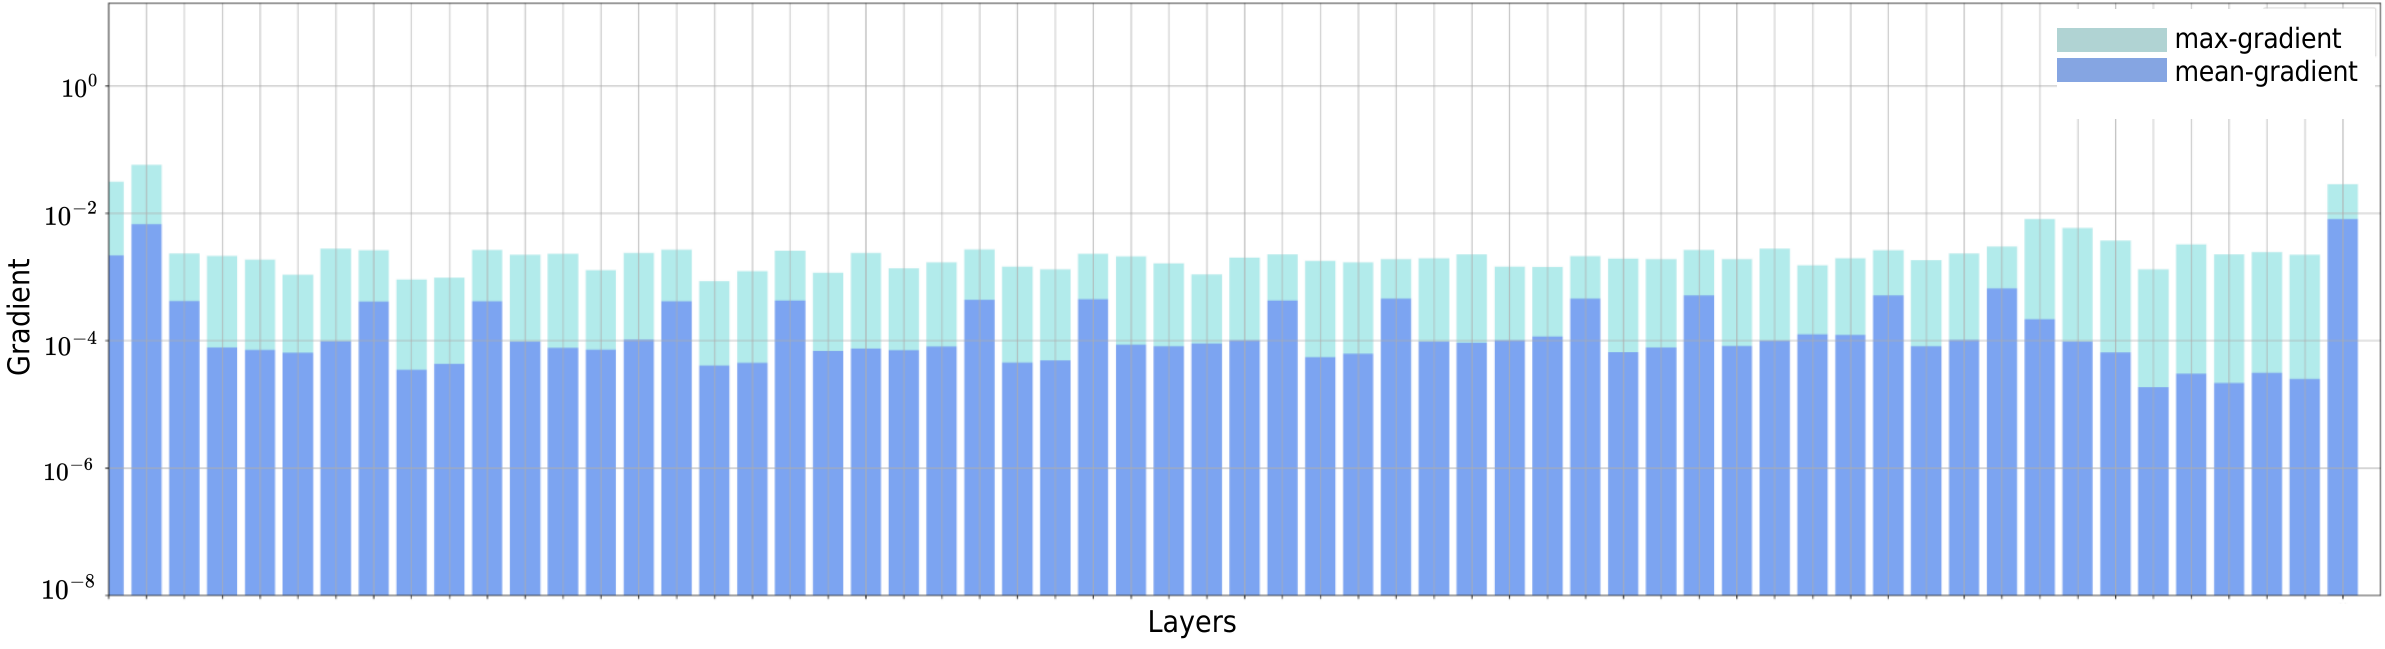
\includegraphics[width=\textwidth]{img/results/t6_epoch3}}
	

	\caption[Gradientes del modelo ESM2(t6)]{Promedio y máximo de gradientes por capa para el modelo ESM2(t6). (a) Representa los gradientes antes del entrenamiento, (b) representa los gradientes después del entrenamiento durante tres \textit{epochs}.}
	\label{fig:t6}
\end{figure}

\begin{figure}[h]
	\centering
	\subfigure[Gráfico de los gradientes por capa antes de entrenar ESM2(t30).]{\label{fig:a}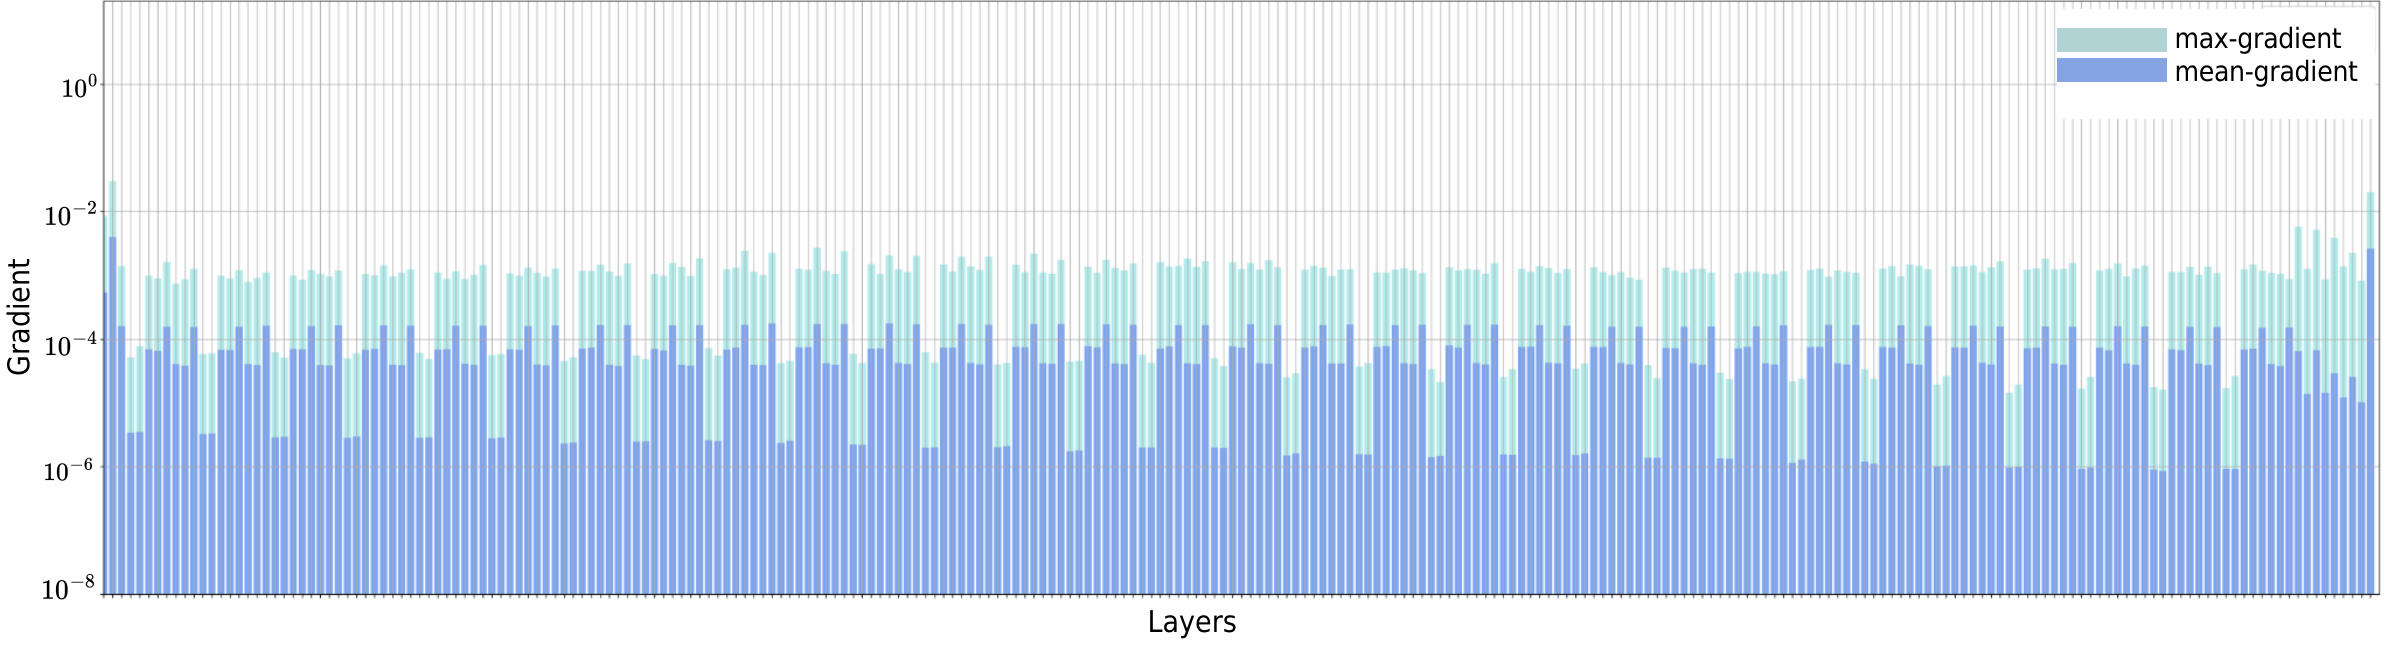
\includegraphics[width=\textwidth]{img/results/t30_epoch0}}
	\subfigure[Gráfico de los gradientes por capa después de entrenar ESM2(t30) durante tres \textit{epochs}.]{\label{fig:b}	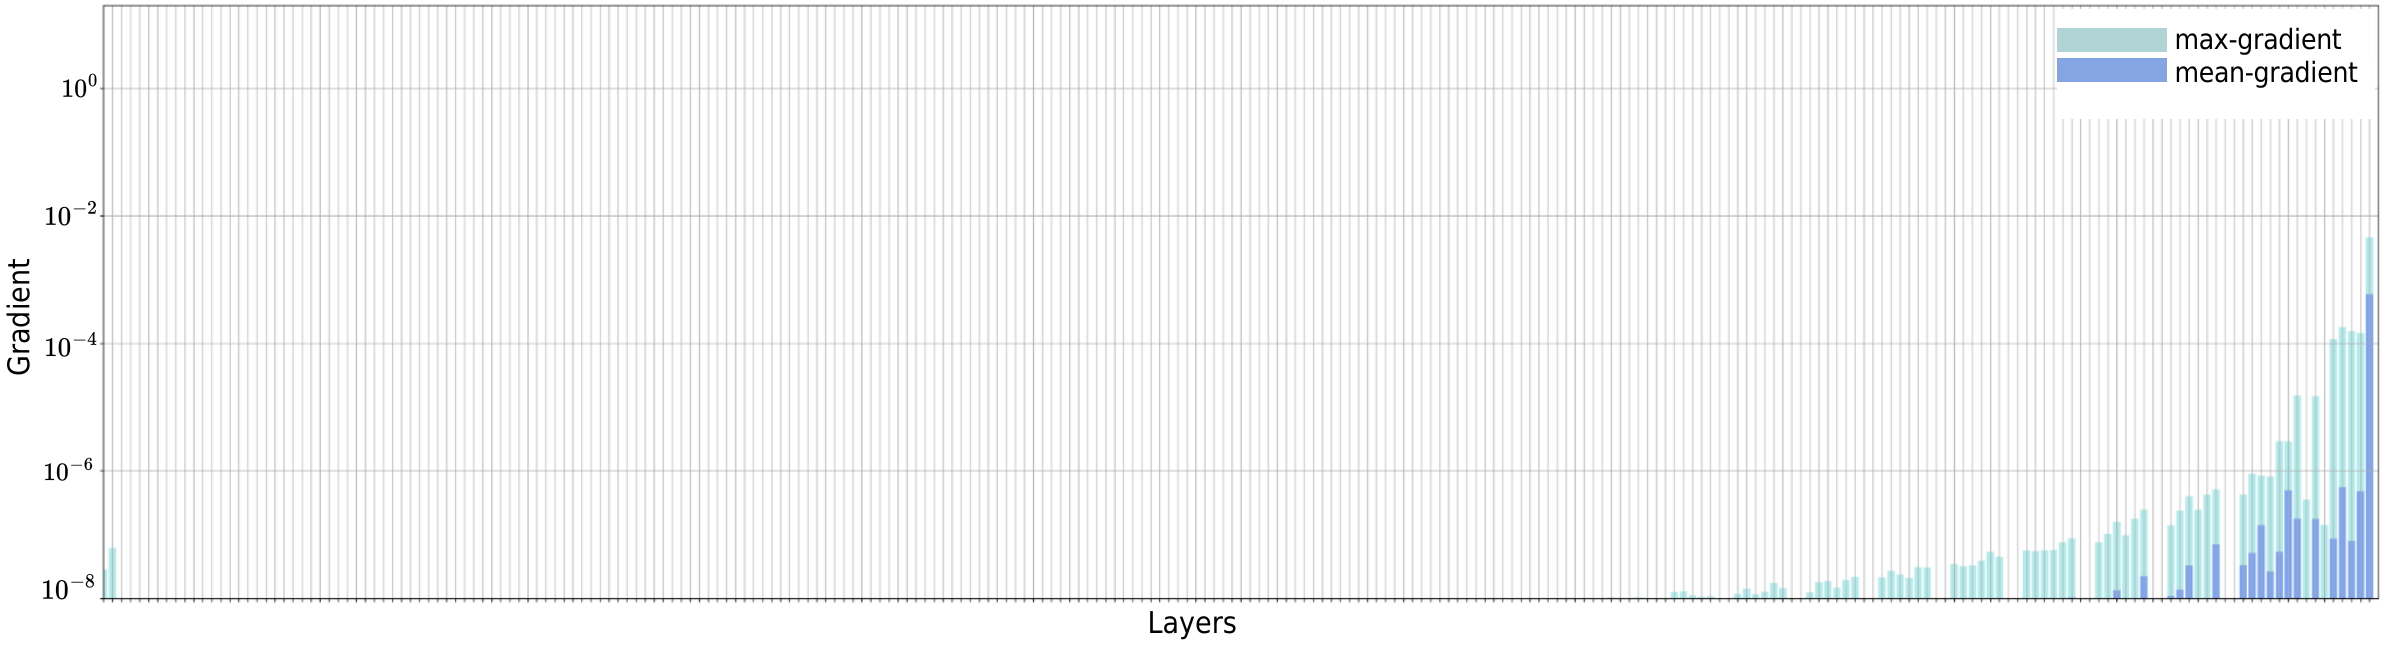
\includegraphics[width=\textwidth]{img/results/t30_epoch3}}
	
	
	\caption[Gradientes del modelo ESM2(t30)]{Promedio y máximo de gradientes por capa para el modelo ESM2(t30). (a) Representa los gradientes antes del entrenamiento, (b) representa los gradientes después del entrenamiento durante tres \textit{epochs}.}
	\label{fig:t30}
\end{figure}


Normalmente, el método de \textit{Gradient Accumulation Steps} (GAS) se utiliza  para reducir el problema de consumo excesivo de memoria de la GPU durante el entrenamiento \citep{zhang2023adam,huang2023measuring}. Sin embargo, esta metodología, puede aliviar ligeramente el problema de \textit{vanish gradient} acumulando gradientes durante algunas iteraciones y solo actualizando el optimizador después de haber realizado un número de iteraciones. Por ejemplo, en la Tabla \ref{tab:comparison_3_epochs}, mostramos los resultados después de aplicar GAS a todos los modelos de \textit{Transformer}, después de entrenar durante tres \textit{epochs}. De estos resultados notamos que los modelos ESM2(t30)-Normal, ESM2(t33)-Normal, TAPE-Normal y ProtBert-Normal no convergieron sin GAS; sin embargo, si los entrenamos con GAS, alcanzaron resultados aceptables.

En particular, la incorporación de\textit{Gradient Accumulation Steps} (GAS) en TAPE-GAS no solo mitiga el problema de \textit{vanish gradient}, sino que también mejora el rendimiento en comparación con otros experimentos que involucran a TAPE, como TAPE-Normal, TAPE-Freeze y TAPE-Freeze-GAS. El mismo fenómeno se observó también en los modelos de ProtBert.


\section{Entrenamiento (30 \textit{epochs})}

Para una comparación más detallada, ampliamos los \textit{epochs} de entrenamiento de los modelos con mejor rendimiento de la Tabla \ref{tab:comparison_3_epochs}, incluyendo ESM2(T6) y TAPE, a 30 \textit{epochs} con \textit{early stopping}. Además, incluimos a ESM2(t30) para investigar si los modelos más grandes logran mejores resultados durante un período de entrenamiento más largo. Cabe señalar que ProtBert-BFD se excluyó del análisis debido a su bajo rendimiento. Como se indica en la Tabla \ref{tab:comparison}, los modelos ESM2 obtienen sus mejores resultados cuando se aplica la metodología de congelación de capas. En cambio, para TAPE, los mejores resultados se logran al utilizar GAS sin congelación. Es importante destacar que TAPE-GAS y ESM2(t6)-Freeze produjeron los resultados más favorables, con TAPE-GAS superando ligeramente a ESM2(t6)-Freeze en este aspecto.

\begin{table*}[]
	\centering
	\caption[Comparación de los modelos \textit{Transformer} entrenados por 30 \textit{epochs}.]{
		Evaluación del rendimiento de los modelos de \textit{Transformer} con \textit{Gradient Accumulation Steps} (GAS) y la metodología de congelación de capas \textbf{entrenados durante treinta (30) \textit{epochs}}. Además, el sufijo 'Normal' representa el entrenamiento clásico utilizando los hiperparámetros de la Sección \ref{sec:fine-tuned}. La inclusión del sufijo 'GAS' en cada modelo indica la integración de \textit{Gradient Accumulation Steps}, mientras que el sufijo 'Freeze' señala nuestra aplicación de la metodología de congelación de capas a los modelos. Además, el guion '-' en cada celda indica que el modelo no pudo converger.}
	\label{tab:comparison}
	\scriptsize
	\setlength{\tabcolsep}{0.5em} % for the horizontal padding
	{\renewcommand{\arraystretch}{1.5}% for the vertical padding
	\begin{tabular}{llllllll} 
		\textbf{}            & \textbf{Accuracy} & \textbf{Precision} & \textbf{Recall} & \textbf{F1-score} & \textbf{AUC}    & \textbf{MCC}    & \textbf{Termino} \\ \midrule
		ESM2(t6)-Normal             & 0.9390            & 0.9333             & \textbf{0.9453} & 0.9392            & 0.9797          & 0.8780          & 9 epochs            \\
		ESM2(t6)-Freeze      & \textbf{0.9401}   & \textbf{0.9398}    & 0.9402          & \textbf{0.9400}   & \textbf{0.9830} & \textbf{0.8802} & 6 epochs            \\
		ESM2(t6)-GAS         & 0.9366            & 0.9322             & 0.9413          & 0.9368            & 0.9818          & 0.8732          & 15 epochs           \\
		ESM2(t6)-Freeze-GAS  & 0.9354            & 0.9326             & 0.9383          & 0.9355            & 0.9813          & 0.8708          & 17 epochs           \\ \midrule
		ESM2(t30)-Normal            & -                 & -                  & -               & -                 & -               & -               & -                   \\
		ESM2(t30)-Freeze     & \textbf{0.9393}   & 0.9304             & \textbf{0.9493} & \textbf{0.9397}   & 0.9787          & \textbf{0.8787} & 14 epochs           \\
		ESM2(t30)-GAS        & 0.9346            & \textbf{0.9337}    & 0.9352          & 0.9345            & 0.9808          & 0.8691          & 17 epochs           \\
		ESM2(t30)-Freeze-GAS & 0.9363            & 0.9319             & 0.9411          & 0.9365            & \textbf{0.9818} & 0.8726          & 27 epochs           \\ \midrule
		TAPE-Normal                 & -                 & -                  & -               & -                 & -               & -               & -                   \\
		TAPE-Freeze          & 0.9395            & \textbf{0.9404}    & 0.9382          & 0.9393            & 0.9815          & 0.8790          & 9 epochs            \\
		TAPE-GAS             & \textbf{0.9415}   & 0.9352             & \textbf{0.9484} & \textbf{0.9418}   & \textbf{0.9841} & \textbf{0.8831} & 5 epochs            \\
		TAPE-Freeze-GAS      & 0.9359            & 0.9297             & 0.9428          & 0.9362            & 0.9820          & 0.8719          & 18 epochs      \\     
	\end{tabular}}
\end{table*}

\section{Comparación con los Métodos del Estado del Arte}

\sloppy
Además, comparamos los mejores modelos, ESM2(t6)-Freeze y TAPE-GAS, entrenados durante 30 \textit{epochs} (consulte la Tabla \ref{tab:comparison}), con métodos de vanguardia. Cubrimos NetMHCpan4.1 \citep{reynisson2020netmhcpan} y MHCFlurry2.0 \citep{o2020mhcflurry} porque son métodos de referencia bien conocidos; y tres herramientas más recientes como Anthem \citep{mei2021anthem}, Acme \citep{hu2019acme} y MixMHCpred2.2 \citep{gfeller2023improved}.

\sloppy
Durante la evaluación de estas herramientas en el conjunto de datos de \textit{testing}, encontramos consideraciones específicas para ACME. Para garantizar una evaluación justa, excluimos los siguientes \textit{alleles} de la evaluación para ACME: HLA-C01:02, HLA-C02:02, HLA-C03:03, HLA-C03:04, HLA-C04:01, HLA-C05:01, HLA-C06:02, HLA-C07:01, HLA-C07:02, HLA-C07:04, HLA-C08:02, HLA-C12:03, HLA-C14:02, HLA-C15:02, HLA-C16:01, HLA-C17:01, HLA-A02:50, HLA-A24:06, HLA-A24:13, HLA-A32:15, HLA-B45:06 y HLA-B83:01. Esta exclusión fue necesaria ya que ACME no pudo predecir la unión péptido-MHC para estos \textit{alleles} particulares. 


Es importante señalar que la elección del umbral para predecir la unión de pMHC puede variar según la herramienta específica y el \textit{k-mer} utilizado. Esta variabilidad hace que el AUC sea una métrica ideal para comparar métodos, ya que proporciona una evaluación robusta que no es sensible a las diferencias de umbral. Por esta razón, en la Figura \ref{fig:comparison_final} y \ref{fig:ROC_comparison_final}, presentamos el AUC y la curva ROC respectivamente de TAPE-GAS, ESM2(t6)-Freeze, NetMHCpan4.1 y MHCFlurry2.0, Anthem, Acme y MixMHCpred2.2. Según estos gráficos, TAPE-GAS y ESM2(t6)-Freeze obtuvieron el valor más alto de AUC.

Además, al evaluar métricas de rendimiento de clasificación binaria, estandarizamos el umbral para TAPE-GAS y ESM2(t6) en 0.5. Mantuvimos un umbral de 0.5 para NetMHCpan4.1, de acuerdo con su configuración recomendada, mientras que para ACME, seguimos un umbral de 0.42, según lo recomendado en su documentación. En el caso de Anthem, la herramienta proporcionó predicciones binarias de unión directamente. Sin embargo, para MixMHCpred2.2 y MHCfurry, determinamos los valores óptimos de umbral a partir del conjunto de datos de \textit{testing}, resultando en 2.7308 y 0.09439, respectivamente. En la Tabla \ref{tab:final_comparison}, presentamos una comparación exhaustiva entre TAPE-GAS y ESM2(t6)-Freeze (entrenados durante 30 \textit{epochs}) y las herramientas del estado del arte. Los resultados demuestran claramente que TAPE-GAS y ESM2(t6)-Freeze superan consistentemente a las herramientas del estado del arte en todas estas métricas: \textit{AUC, precisión, recall, F1-score} y \textit{MCC}.

\begin{figure}
	\centering
	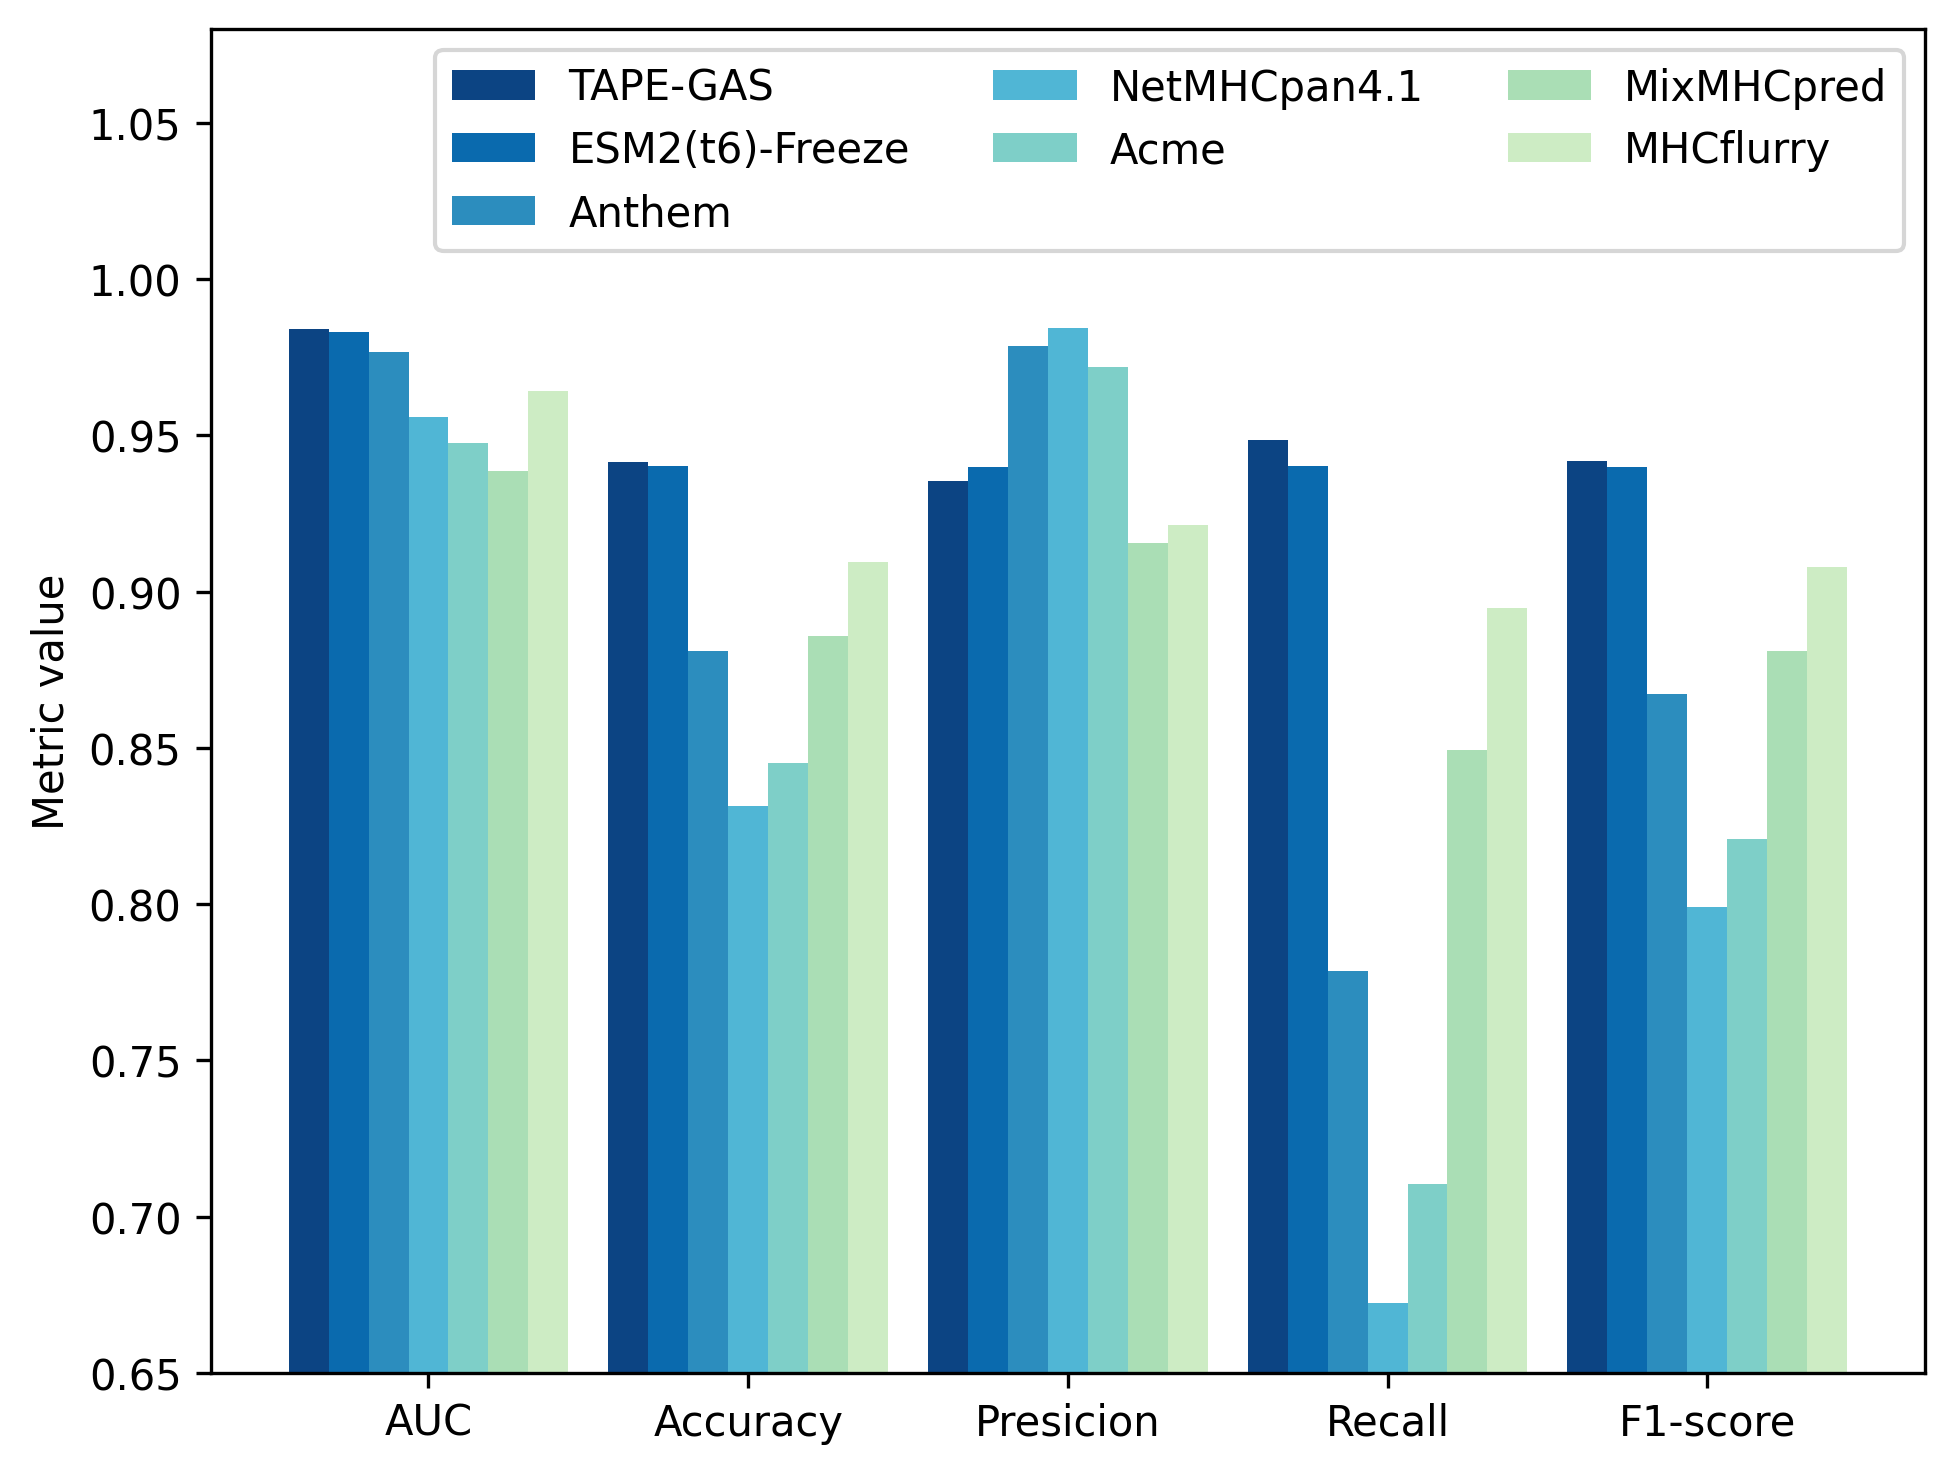
\includegraphics[width=0.8\textwidth]{img/results/metrics_comparison}
	\caption[Comparación del AUC con métodos del estado del arte]{Los valores de AUC para TAPE-GAS y ESM2(t6) entrenados durante 30 epochs, en comparación con las herramientas de vanguardia.}
	\label{fig:comparison_final}
\end{figure}

\begin{figure}
	\centering
	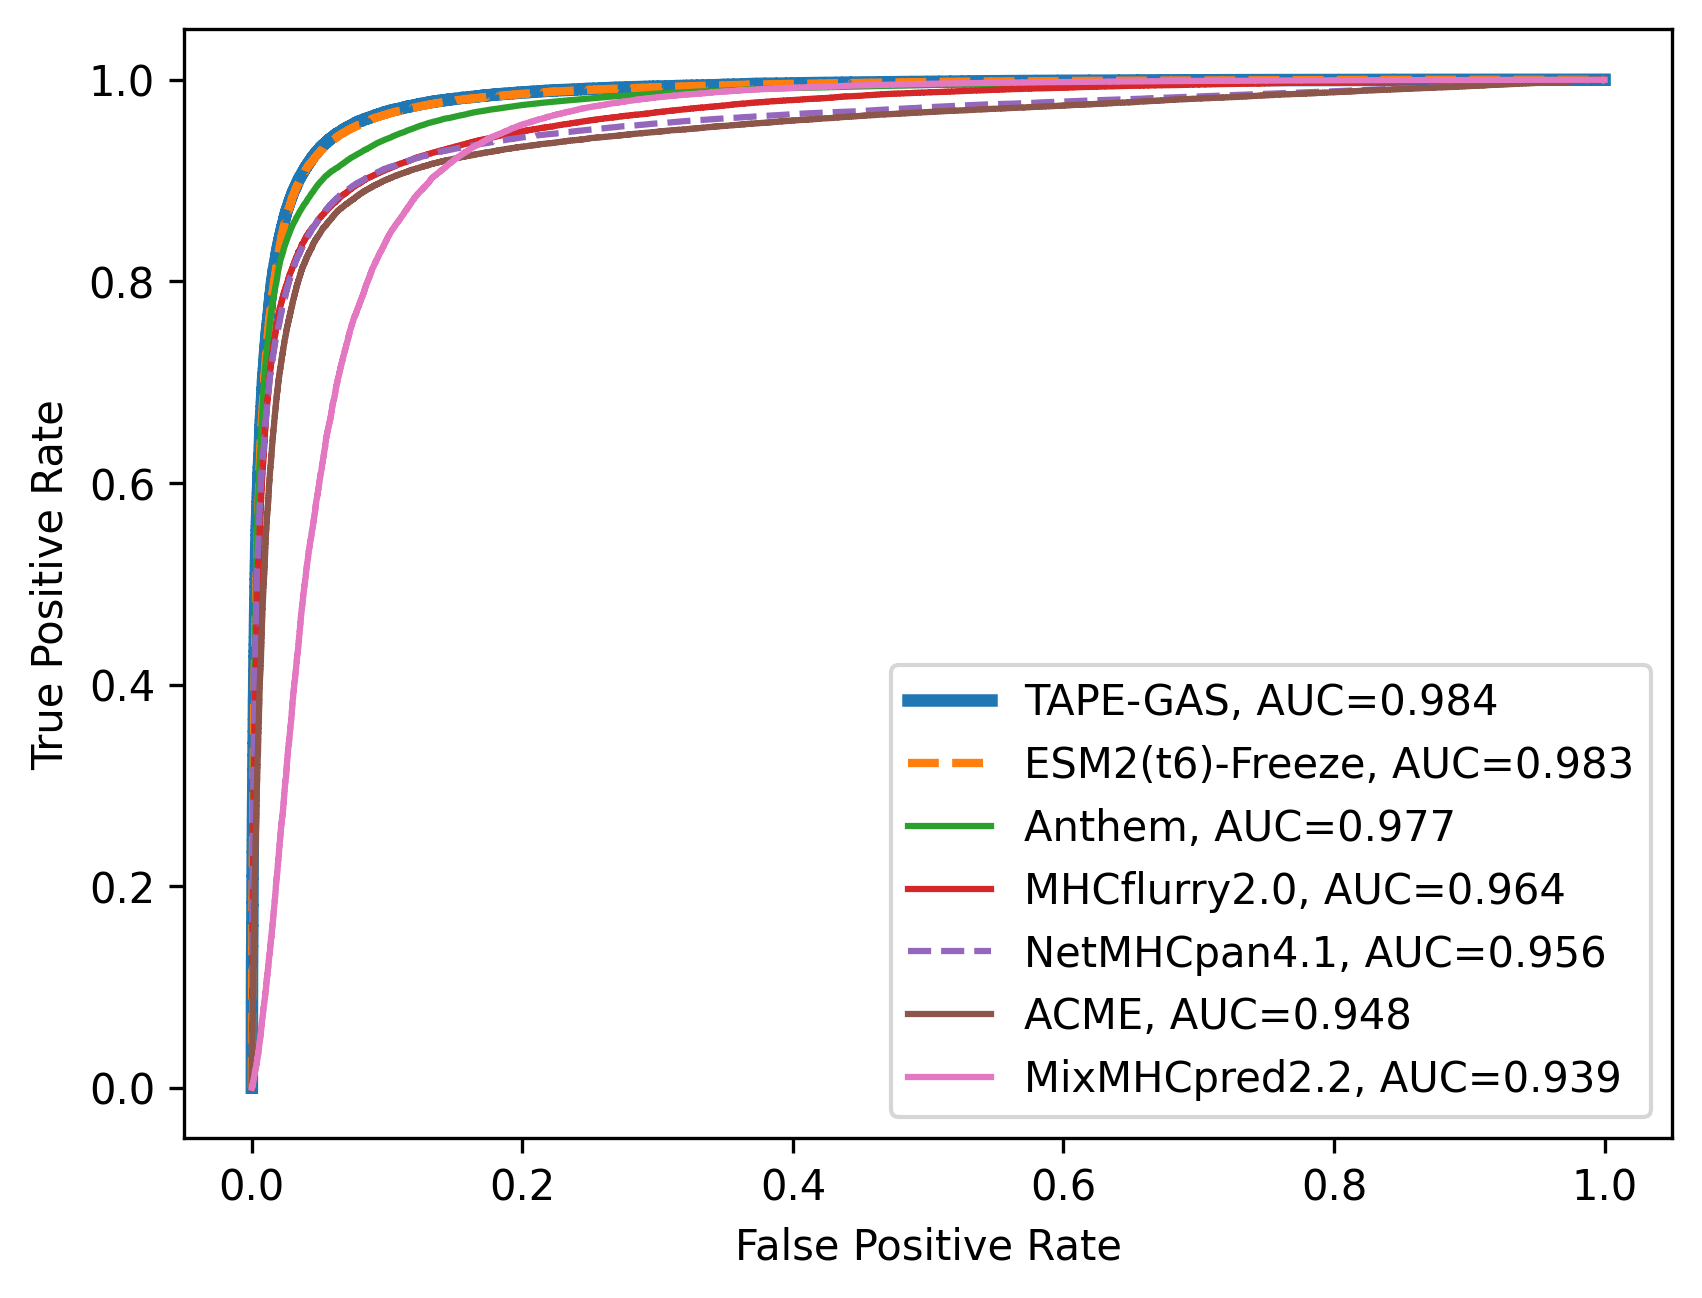
\includegraphics[width=0.8\textwidth]{img/results/ROC_comparison}
	\caption[Comparación de ROC con métodos del estado del arte]{Las curvas ROC para TAPE-GAS y ESM2(t6) entrenados durante 30 epochs, en comparación con las herramientas de vanguardia.}
	\label{fig:ROC_comparison_final}
\end{figure}

\begin{table}[]
	\centering
	\caption{Evaluación del desempeño de los modelos de \textit{Transformer} TAPE-GAS y ESM2(t6)-Freeze, entrenados durante 30 \textit{epochs}, en comparación con Anthem, NetMHCpan4.1, ACME, MixMHCpred2.2 y MhcFlurry2.0.}
	\label{tab:final_comparison}
	\footnotesize
	\setlength{\tabcolsep}{0.5em} % for the horizontal padding
	{\renewcommand{\arraystretch}{1.5}% for the vertical padding
	\begin{tabular}{lllllll}
		& \textbf{Accuracy} & \textbf{Precision} & \textbf{Recall} & \textbf{F1-score} & \textbf{AUC}    & \textbf{MCC}    \\ \midrule
		TAPE-GAS        & \textbf{0.9415}   & 0.9352             & \textbf{0.9484} & \textbf{0.9418}   & \textbf{0.9841} & \textbf{0.8831} \\
		ESM2(t6)-Freeze & \textbf{0.9401}   & 0.9398             & \textbf{0.9402} & \textbf{0.9400}   & \textbf{0.9830} & \textbf{0.8802} \\
		
		Anthem          & 0.8811            & \textbf{0.9786}    & 0.7787          & 0.8673            & 0.9768          & 0.7785          \\
		NetMHCpan4.1    & 0.8312            & \textbf{0.9844}    & 0.6724          & 0.7991            & 0.9557          & 0.6982          \\
		
		ACME            & 0.8452            & 0.9717             & 0.7105          & 0.8208            & 0.9476          & 0.7165          \\
		MixMHCpred2.2   & 0.8857            & 0.9155             & 0.8493          & 0.8811            & 0.9386          & 0.7733          \\
		MhcFlurry2.0    & 0.9093            & 0.9211             & 0.8948          & 0.9078            & 0.9642          & 0.8189 \\         
	\end{tabular}}
\end{table}

Finalmente, mostramos la distribución de AUC para TAPE-GAS y ESM2(t6)-Freeze, ambos entrenados durante 30 épocas, junto con Anthem, NetMHCpan4.1, ACME, MixMHCpred2.2 y MHCflurry2.0. En este caso, evaluamos cada distribución por \textit{k-mer} (Figura \ref{fig:auc_distribution}, \ref{fig:auc_distribution2} y \ref{fig:auc_distribution14}). En todos los \textit{k-mer}, TAPE-GAS y ESM2(t6)-Freeze presentan la puntuación más alta. Además, es importante destacar que el modelo pequeño ESM2(t6)-Freeze ofrece resultados superiores para péptidos más largos con longitudes de 11, 12, 13 y 14.



\begin{figure}[H]
	\centering	
	\subfigure[8-mer]{\label{fig:a}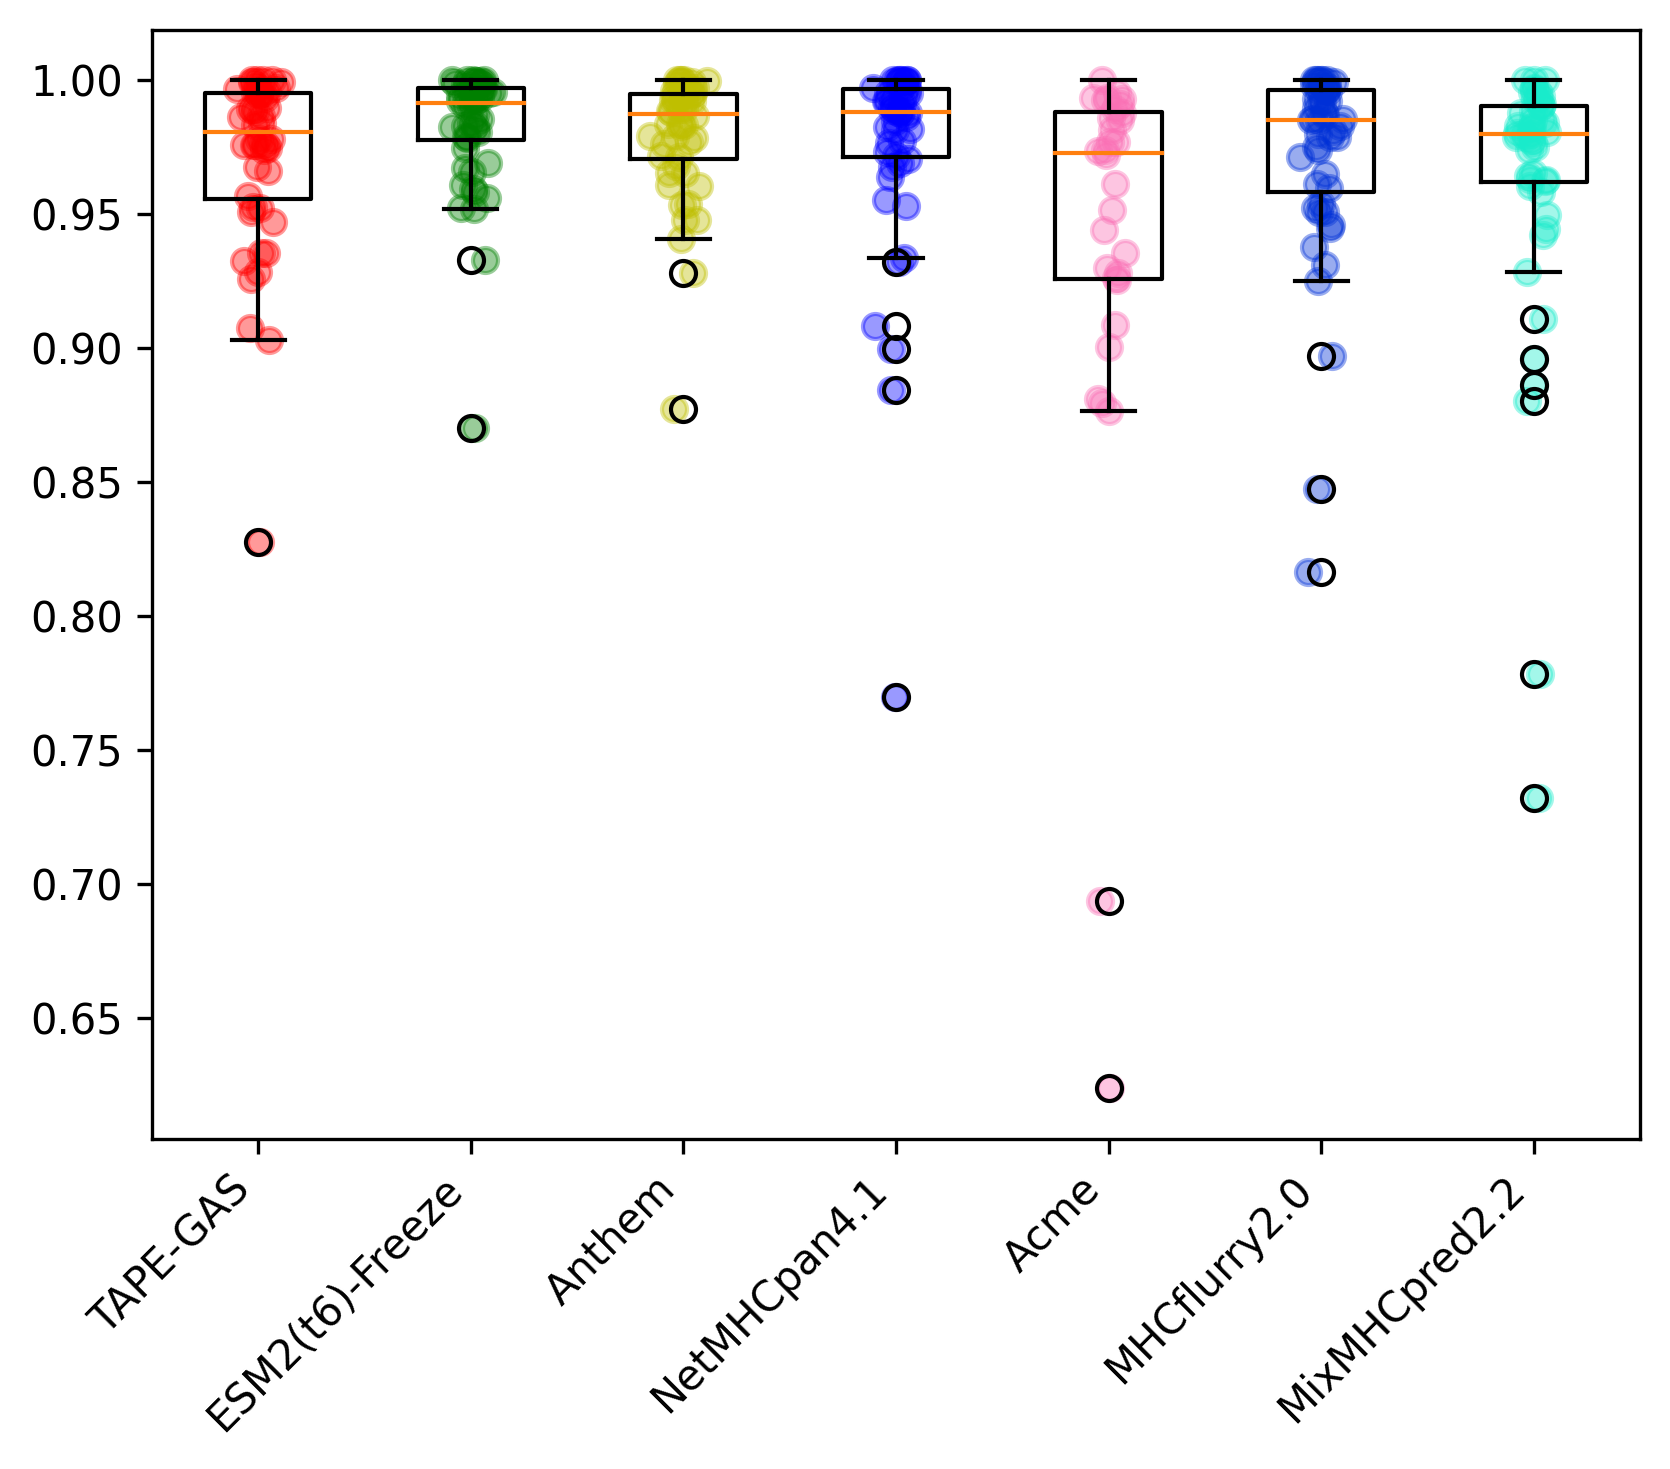
\includegraphics[width=0.49\textwidth]{img/results/auc_distribution_8-mer}}
	\subfigure[9-mer]{\label{fig:a}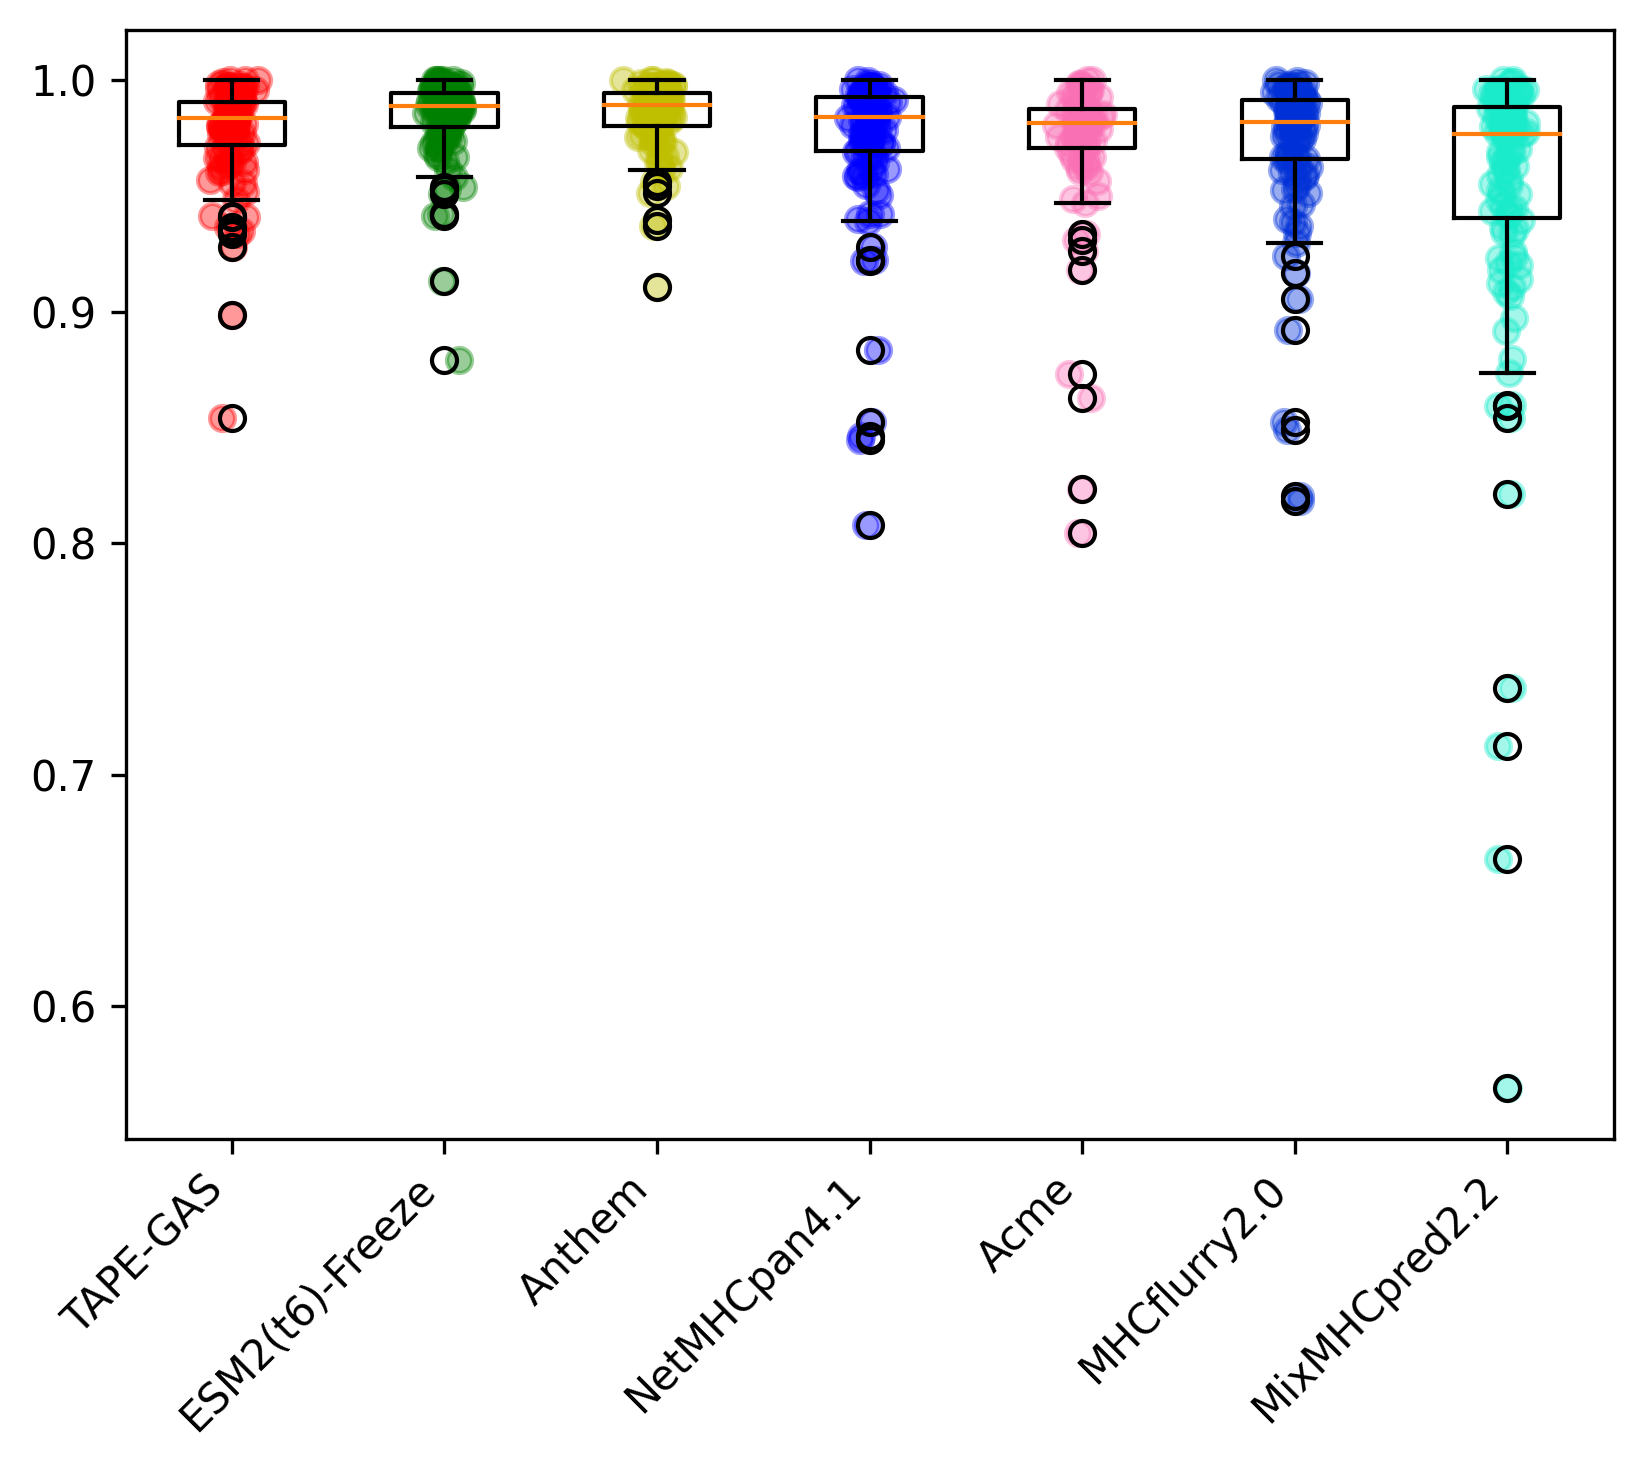
\includegraphics[width=0.49\textwidth]{img/results/auc_distribution_9-mer}}
	\subfigure[10-mer]{\label{fig:a}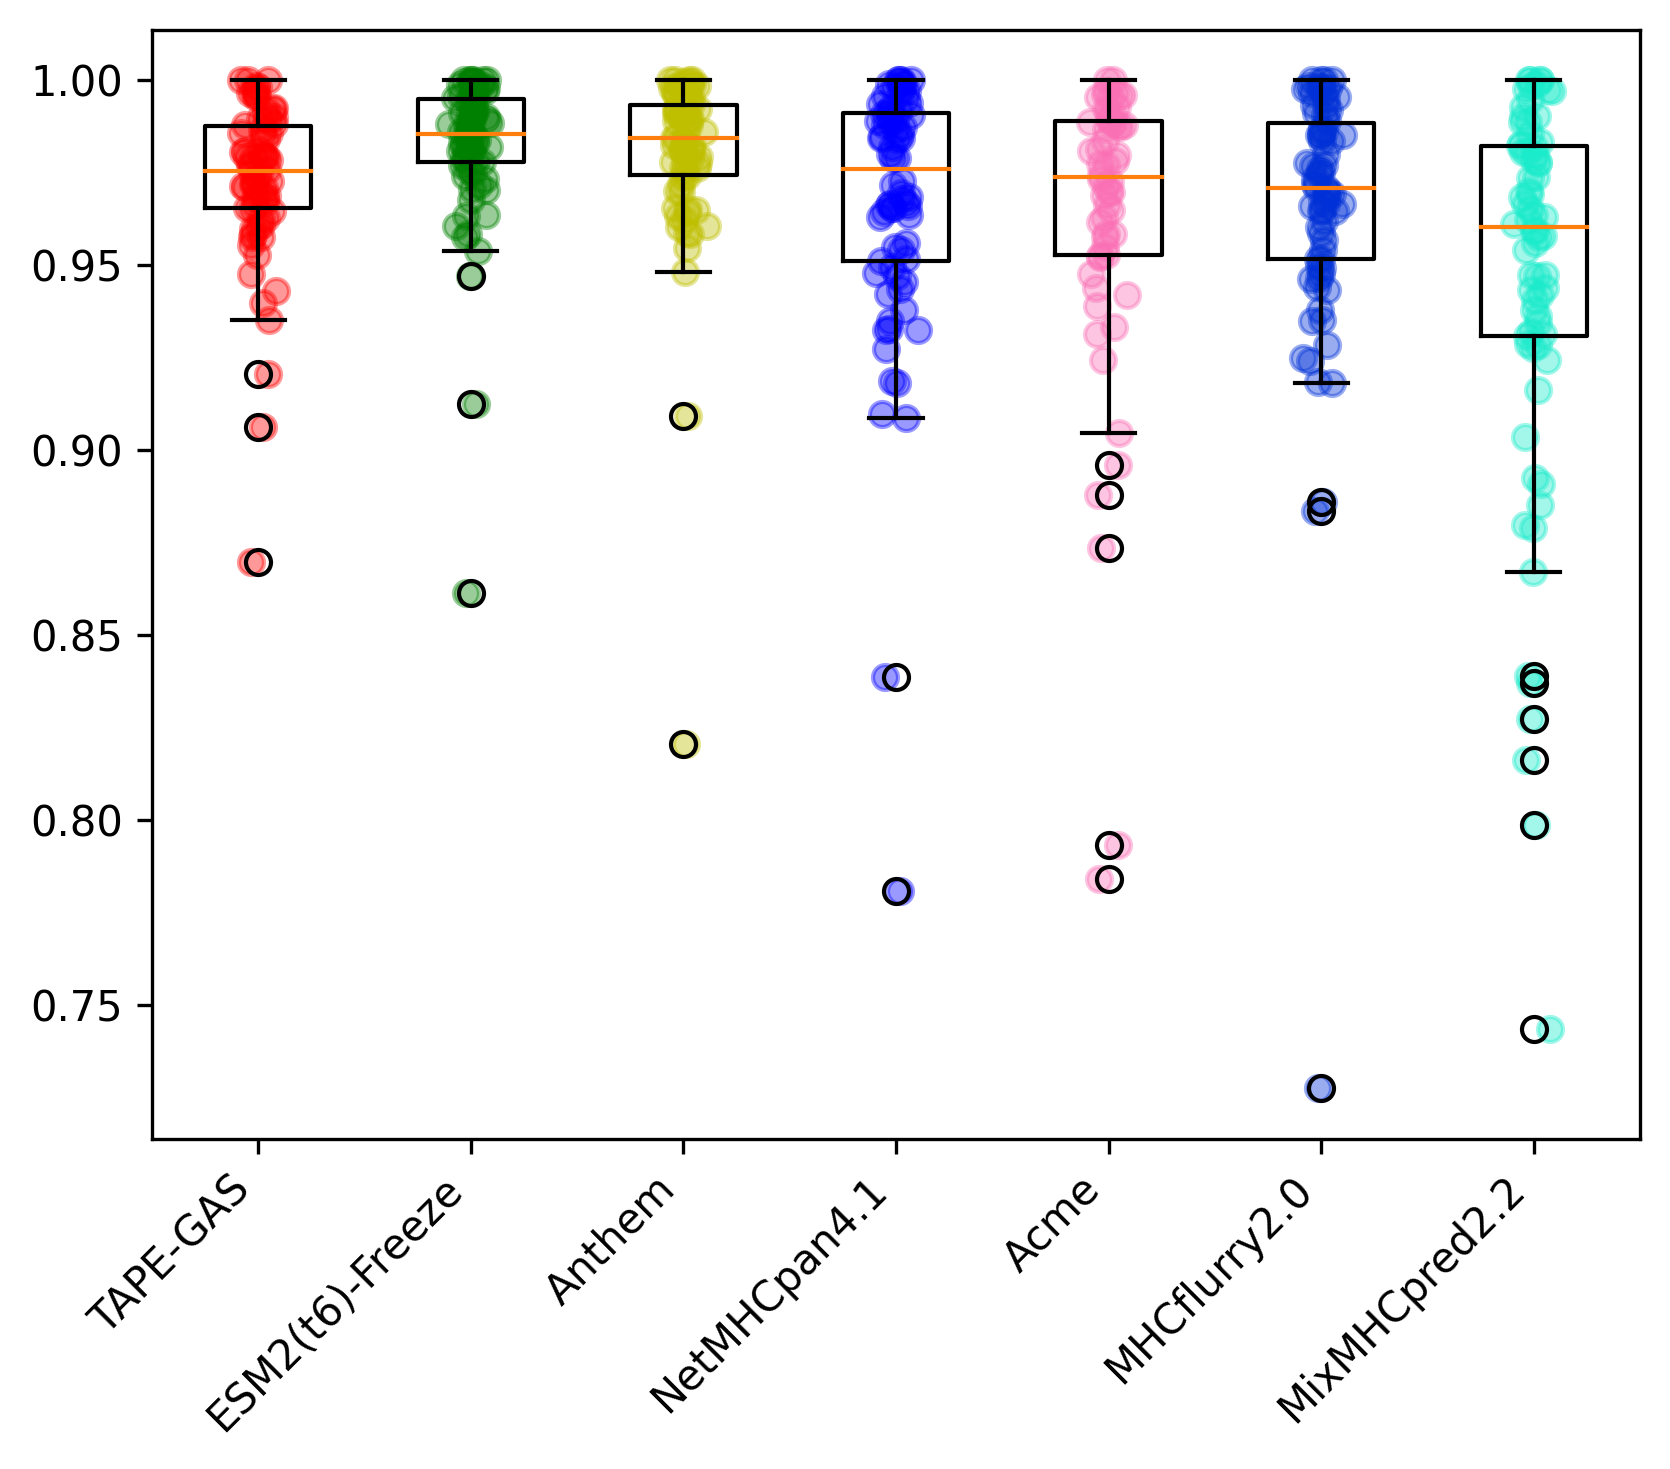
\includegraphics[width=0.49\textwidth]{img/results/auc_distribution_10-mer}}
	\subfigure[11-mer]{\label{fig:a}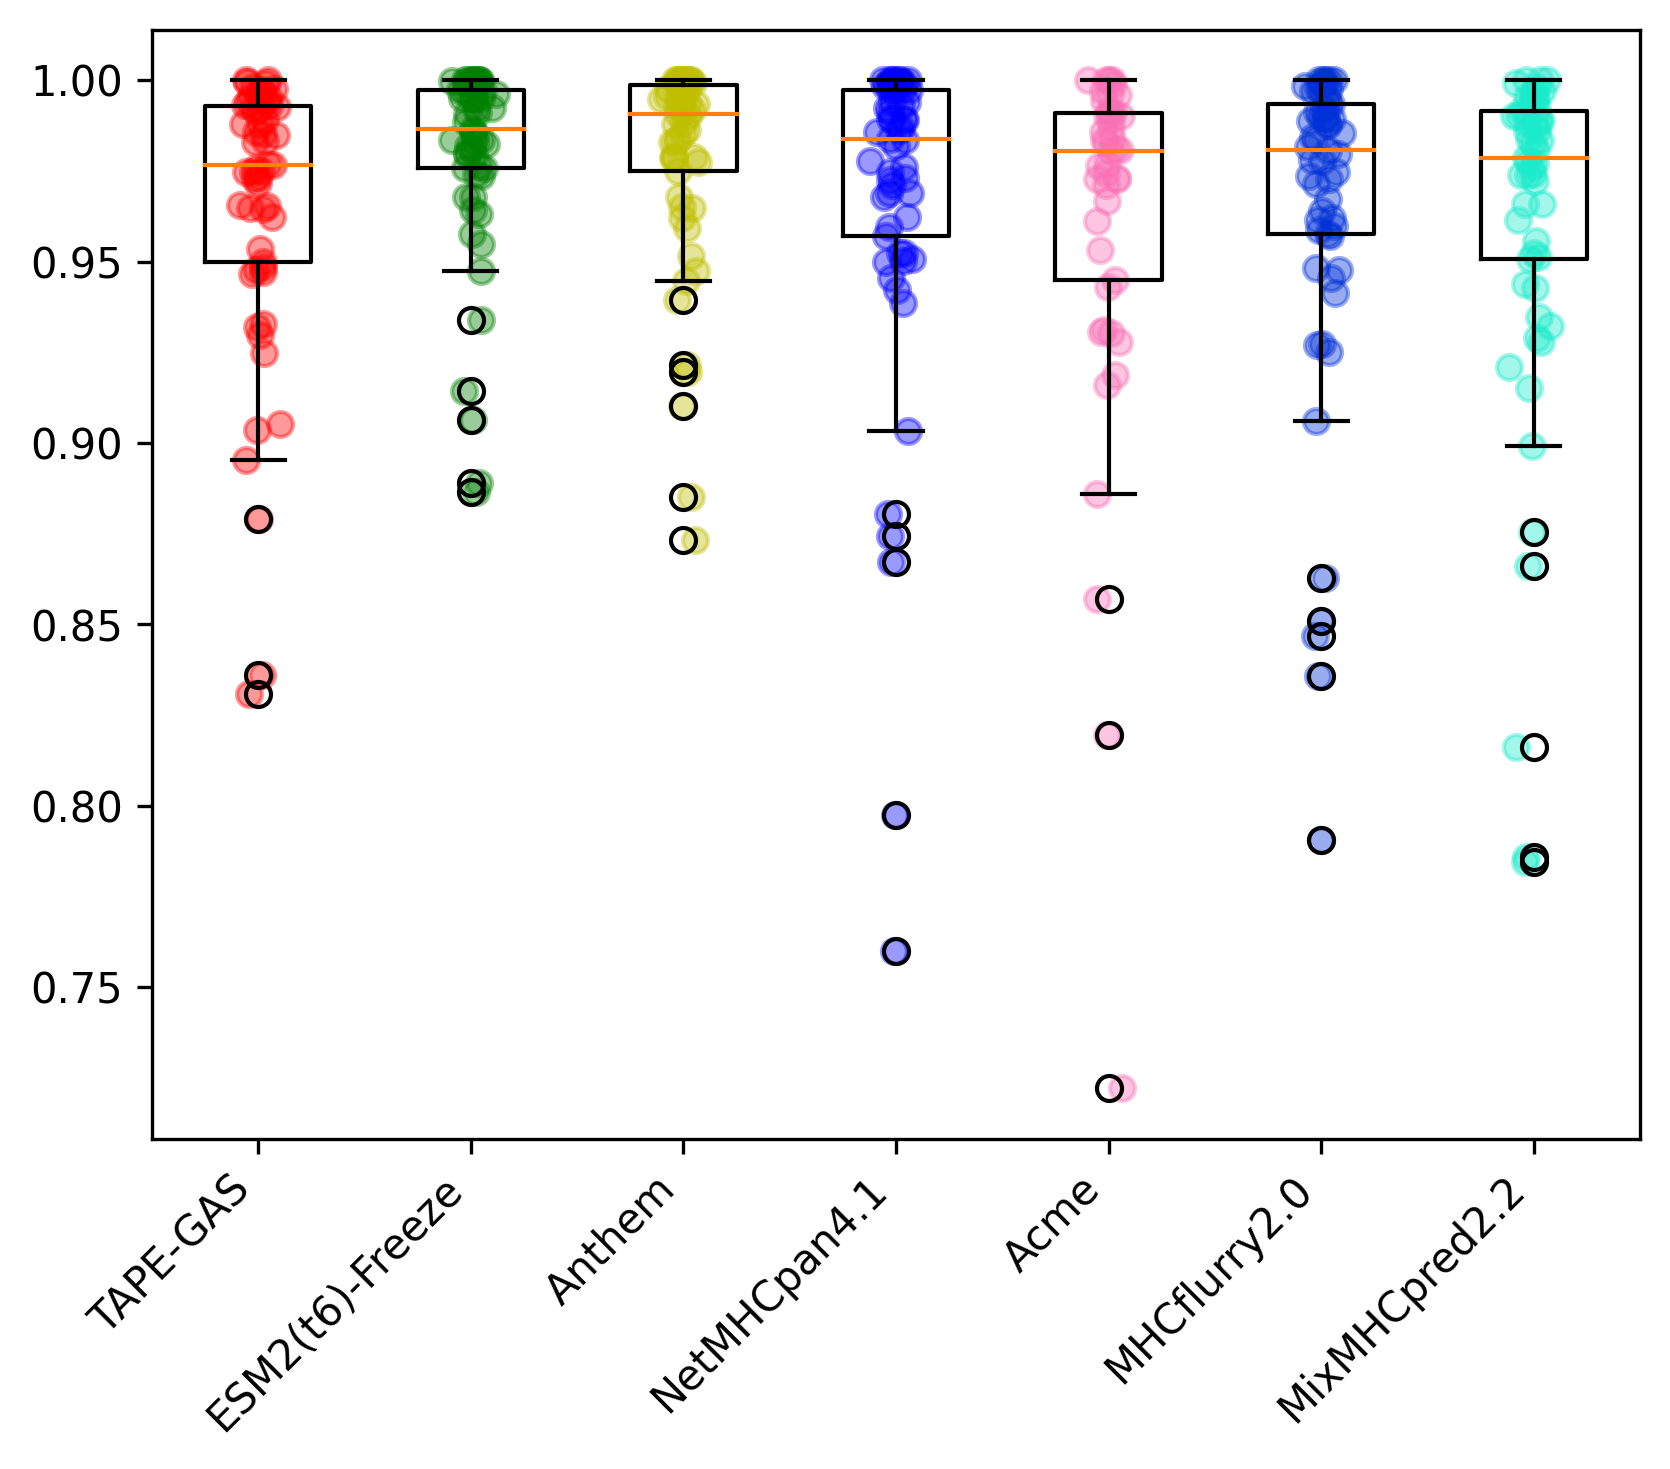
\includegraphics[width=0.49\textwidth]{img/results/auc_distribution_11-mer}}
	
		
	\caption{
		La distribución de AUC para TAPE-GAS y ESM2(t6)-Freeze, ambos entrenados durante 30 \textit{epochs} para 8, 9, 10 y 11-mers; junto con Anthem, NetMHCpan4.1, ACME, MixMHCpred2.2 y MHCflurry2.0.}
	\label{fig:auc_distribution}
\end{figure}

\begin{figure}[H]
	\centering	

	\subfigure[12-mer]{\label{fig:a}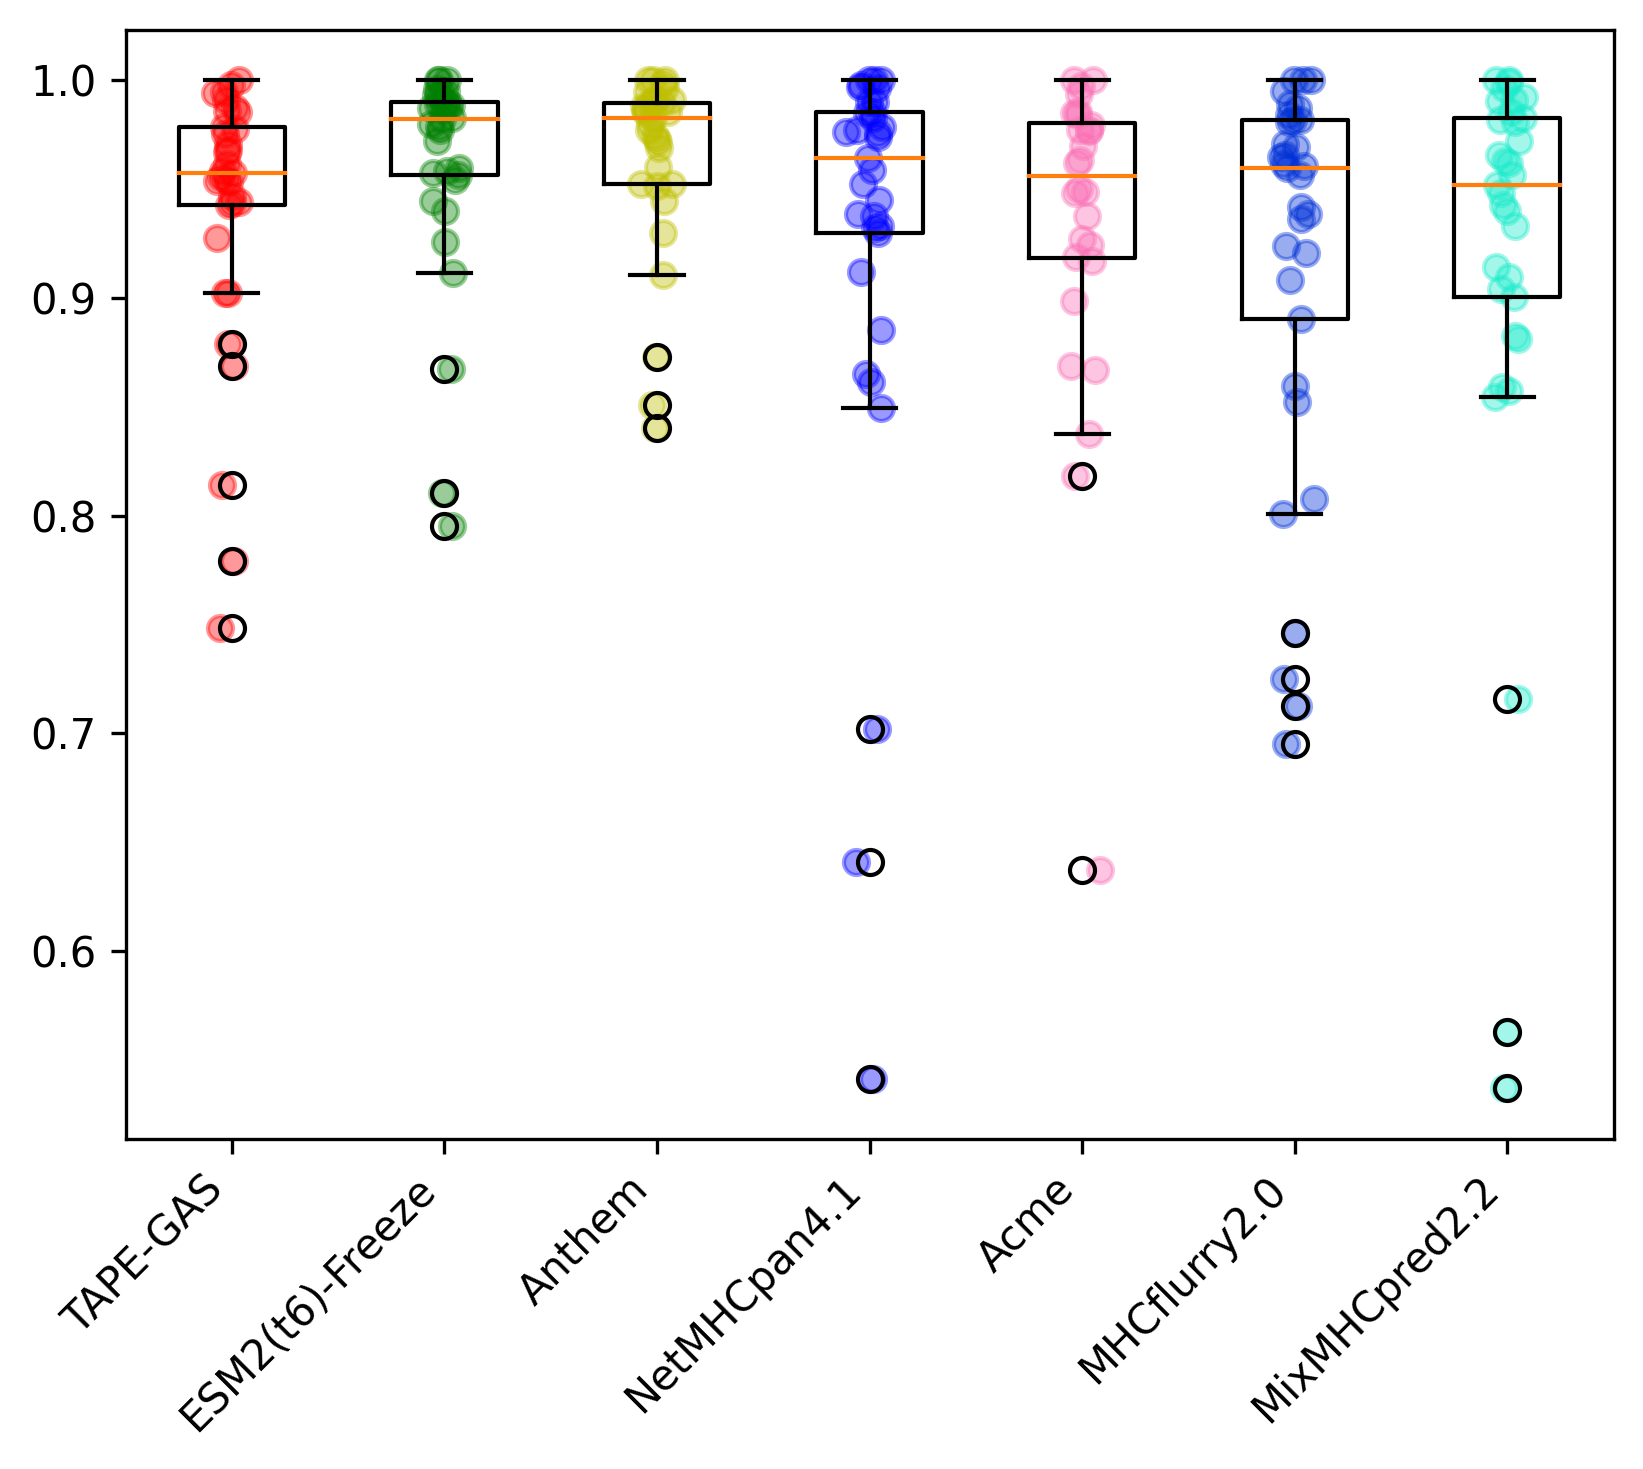
\includegraphics[width=0.49\textwidth]{img/results/auc_distribution_12-mer}}
	\subfigure[13-mer]{\label{fig:a}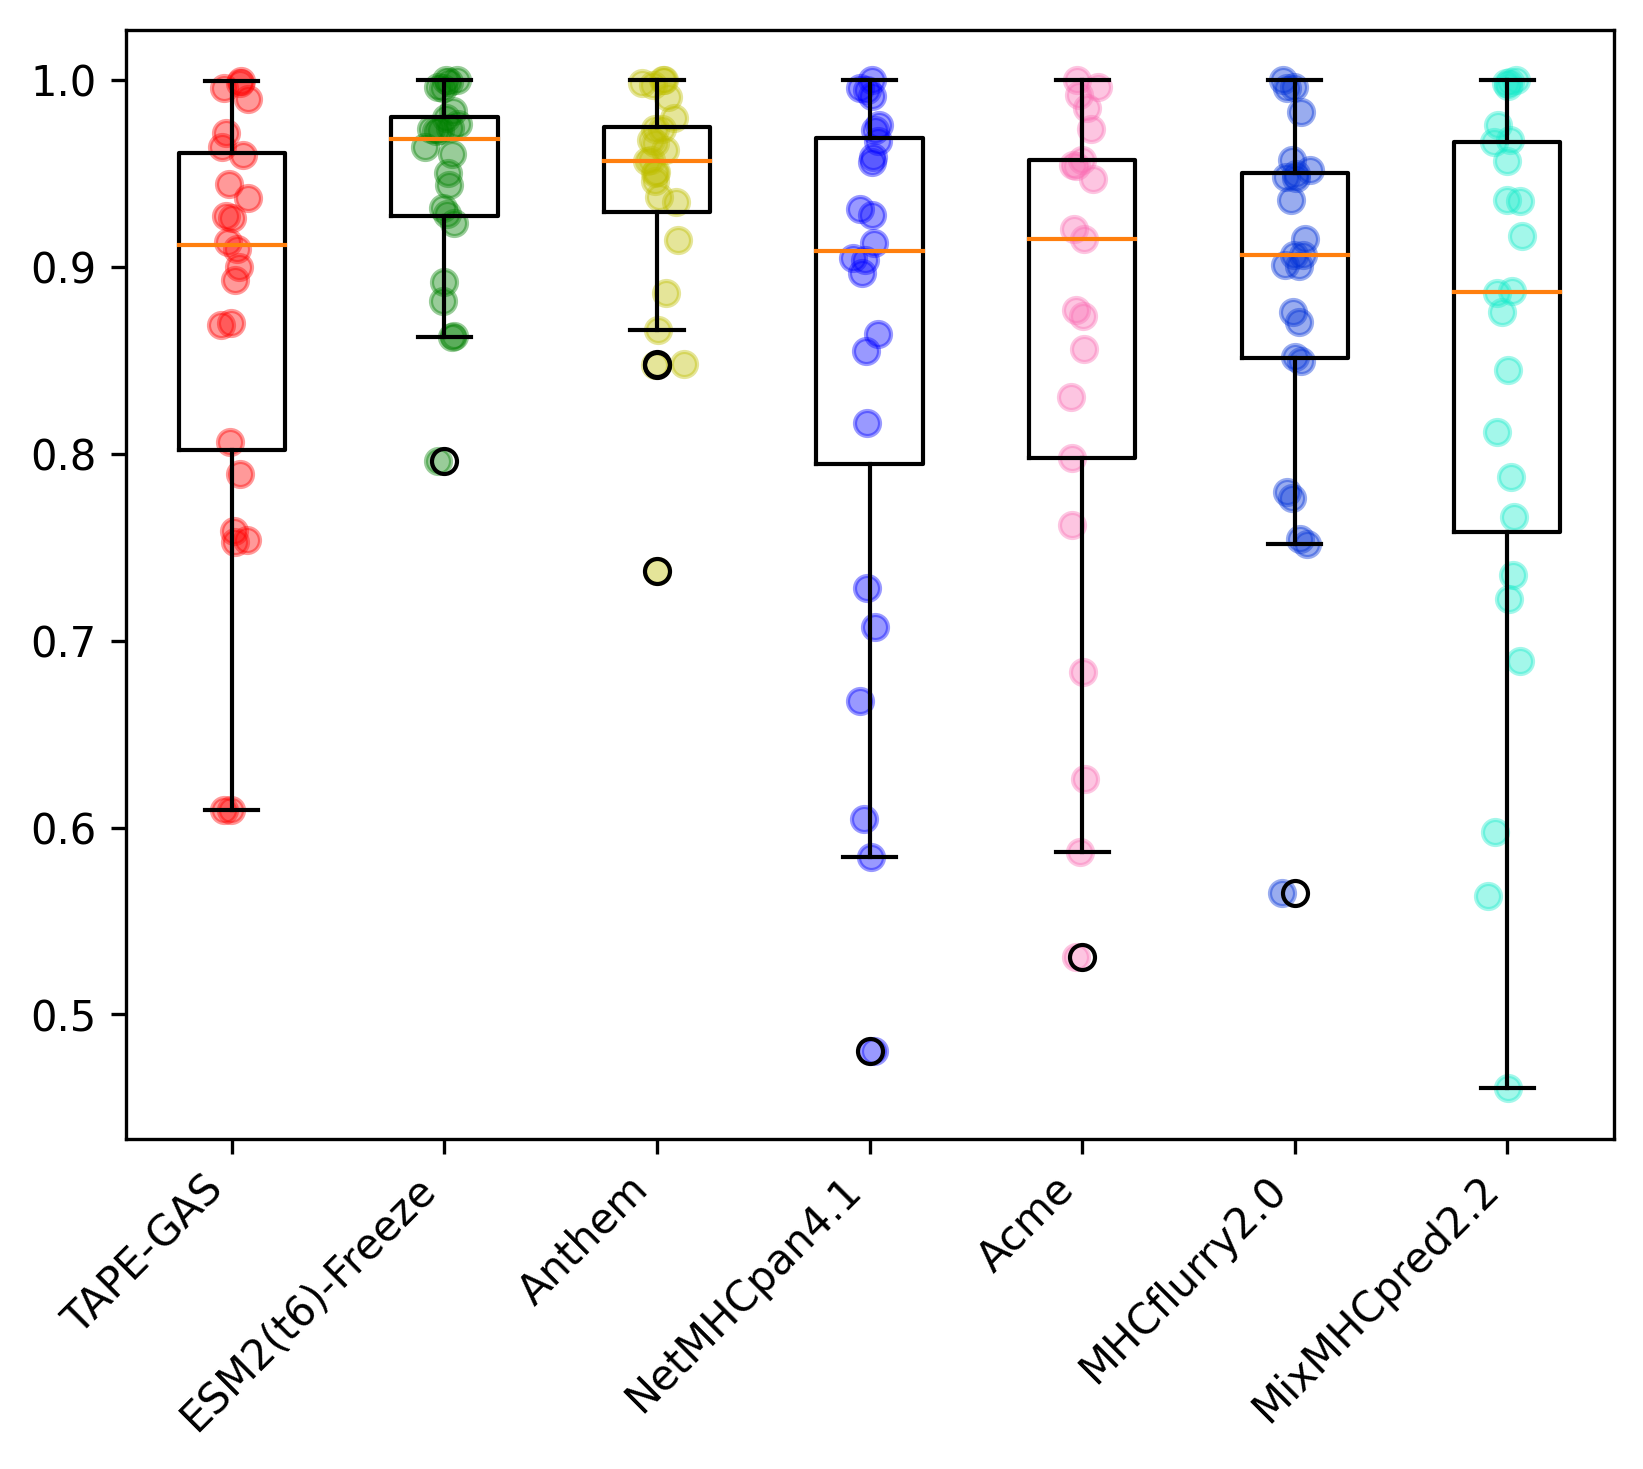
\includegraphics[width=0.49\textwidth]{img/results/auc_distribution_13-mer}}
	
	\caption{
		La distribución de AUC para TAPE-GAS y ESM2(t6)-Freeze, ambos entrenados durante 30 \textit{epochs} para 12 y 13-mers; junto con Anthem, NetMHCpan4.1, ACME, MixMHCpred2.2 y MHCflurry2.0.}
	\label{fig:auc_distribution2}
\end{figure}



\begin{figure}[H]
	\centering	
	\subfigure[14-mer]{\label{fig:a}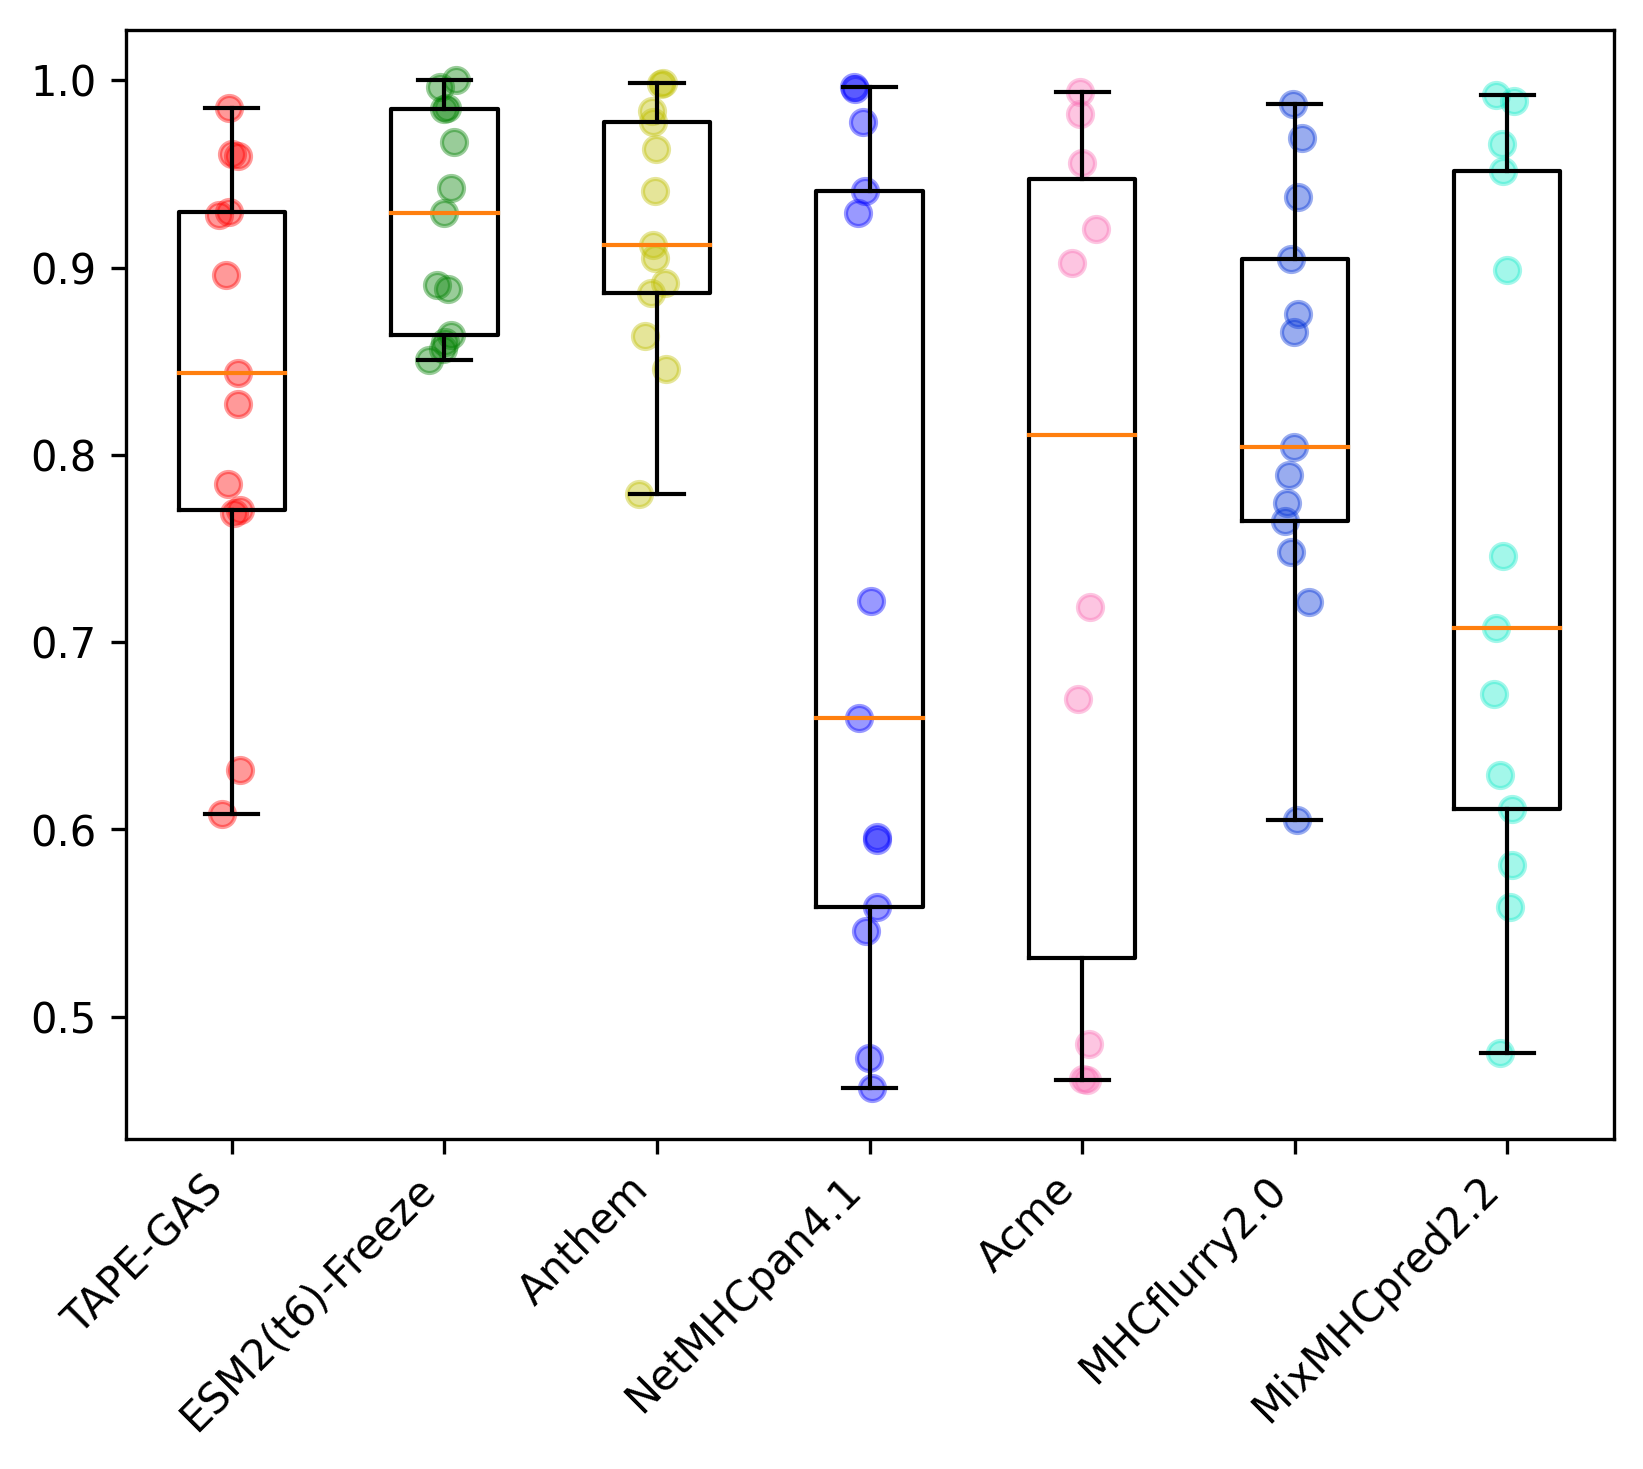
\includegraphics[width=0.49\textwidth]{img/results/auc_distribution_14-mer}}	
	
	\caption{
		La distribución de AUC para TAPE-GAS y ESM2(t6)-Freeze, ambos entrenados durante 30 \textit{epochs} para los péptidos 14-mer; junto con Anthem, NetMHCpan4.1, ACME, MixMHCpred2.2 y MHCflurry2.0.}
	\label{fig:auc_distribution14}
\end{figure}


\section{Herramienta para Predicción de la Unión pMHC}

En base a los resultados obtenidos se ha desarrollado una herramienta de linea de comandos. En esta herramienta podemos hacer predicciones de los modelos con mejor desempeño desarrollados en esta tesis: ESM2(t6)-Freeze y TAPE-GAS, para la predicción de la unión pMHC. Además, tambien podemos reentrenar estos modelos con otras bases de datos. La herramienta es código libre y esta en este repositorio: \href{https://github.com/arceda/pmhc}{https://github.com/arceda/pmhc}.




\section{Discusión}

\subsection{\textit{Fine-tuning} ESM2}

Cuando se consideran específicamente los modelos \textit{Transformer} de ESM2, los resultados más favorables se obtuvieron con el modelo más pequeño, ESM2(t6), como se indica en la Tabla \ref{tab:comparison_3_epochs}. Sin embargo, es importante destacar que los autores de ESM2 informaron en su artículo que, para diversas otras tareas, modelos más grandes como ESM2(t30) y ESM2(t33) superaron a los más pequeños como ESM2(t6) y ESM2(t12) \citep{lin2023evolutionary}. Además, está bien establecido que los modelos más grandes tienden a aprender más rápido pero requieren conjuntos de datos de entrenamiento más extensos \citep{elnaggar2021prottrans}. En el caso de la predicción de la unión pMHC-I, nuestro estudio empleó un conjunto de datos que consta de 559,019 muestras, que no consideramos lo suficientemente grande para ESM2(t33), un modelo que cuenta con 650 millones de parámetros. En futuras investigaciones, planeamos evaluar el rendimiento de modelos más grandes utilizando conjuntos de datos más extensos.

Otra razón potencial para el rendimiento superior de ESM2(t6) podría atribuirse al uso de \textit{Rotary Position Embedding} (RoPE) (RoPE) en lugar de la codificación posicional absoluta. Si bien RoPE puede llevar a un ligero aumento en el costo de entrenamiento, se ha observado que mejora la calidad de los resultados, especialmente para modelos más pequeños \citep{lin2023evolutionary}.

\subsection{Congelamiento de Capas y GAS}
Durante el entrenamiento de los modelos \textit{Transformer}, exploramos la implementación de una metodología de congelación de capas. Este enfoque implica bloquear el modelo \textit{Transformer} mientras se actualizan solo los parámetros de BiLSTM. Como se informa en varios estudios sobre metodologías de congelación en \textit{Transformers} \citep{merchant2020happens,lee2019would,kovaleva2019revealing}, este método generalmente es adecuado para acelerar el proceso de entrenamiento, aunque puede implicar un ligero sacrificio en el desempeño. Sorprendentemente, para los modelos ESM2, esta metodología arrojó los mejores resultados, mientras que para TAPE y ProtBert-BFD, produjo los resultados esperados (ver Tabla \ref{tab:comparison_3_epochs}).


Además, nos encontramos con un problema recurrente de \textit{vanish gradient} al entrenar modelos grandes como TAPE-normal, ProtBert-normal, ESM2(t30)-normal y ESM2(t33)-normal (ver Tabla \ref{tab:comparison_3_epochs}). Este desafío es un fenómeno común al entrenar modelos de lenguaje grandes, ya que los gradientes tienden a acercarse a valores cercanos a cero después de varias etapas de entrenamiento. Para abordar esto, evaluamos la efectividad de emplear \textit{Gradient Accumulation Steps} (GAS). Este método está diseñado para reducir el consumo de memoria durante el entrenamiento acumulando gradientes durante un cierto número de  iteraciones antes de actualizar los parámetros del modelo. En los experimentos, adoptamos la técnica de acumular gradientes durante 64 y 128 iteraciones. Esta técnica alivia ligeramente el problema de gradientes que desaparecen al evitar que los gradientes disminuyan hasta valores cercanos a cero, como se informa para los modelos: ESM2(t30)-GAS, ESM2(t33)-GAS, TAPE-GAS y ProtBert-GAS en la Tabla \ref{tab:comparison_3_epochs}. Sin embargo, es importante tener en cuenta que esta técnica principalmente extiende la cantidad de iteraciones de entrenamiento que se pueden realizar antes de que el modelo posiblemente vuelva a enfrentar el problema de \textit{vanish gradient}. Como ejemplo, al entrenar ProtBert-Normal, las gradientes se acercaban a cero, después del primer \textit{epoch}. Sin embargo, con la introducción de GAS (ProtBert-GAS), logramos extender el entrenamiento a tres \textit{epochs} antes de volver a enfrentar el problema de \textit{vanish gradients}, que resurgió después de cuatro \textit{epochs}.


\subsection{TAPE, ProtBert-BFD y ESM2}

En esta investigación comparamos el desempeño de TAPE, ProtBert-BFD y ESM2, cada uno de los cuales se describe en la Tabla \ref{tab:pretrained}. Las métricas se presentan en la Tabla \ref{tab:comparison_3_epochs}. Según esta información, ProtBert-BFD obtuvo el peor resultado a pesar de que este modelo fue pre-entrenado con el conjunto de datos más grande, BFD, que contiene 2122 millones de muestras y tiene 420 millones de parámetros. Creemos que este resultado se debe a la ruido en las muestras y a los errores en las secuencias en el conjunto de datos BFD \citep{elnaggar2021prottrans}. Además, los modelos \textit{Transformer} grandes requieren más datos para el entrenamiento \citep{elnaggar2021prottrans}, y en nuestro caso este modelo se entreno con 559,019 muestras.


Además, es destacable que TAPE logró los mejores resultados, con ESM2(t6) siguiendo de cerca (como se muestra en la Tabla \ref{tab:comparison_3_epochs}). Los modelos TAPE fueron pre-entrenados utilizando el conjunto de datos Pfam, que es el conjunto de datos más pequeño en esta comparación, con aproximadamente 30 millones de muestras. Es importante mencionar que el conjunto de datos Pfam se deriva de UniProtKB y selectivamente incluye secuencias que pertenecen a \textit{Reference Proteomes} en lugar de abarcar toda la base de datos de UniProtKB \cite{finn2016pfam}. En consecuencia, Pfam cubre la mitad de las secuencias de proteínas en comparación con otros conjuntos de datos basados en UniProtKB, pero sus muestras son de mayor calidad. Por lo tanto, es lógico suponer que TAPE encapsula una representación más completa y refinada de la información de proteínas en comparación con otros modelos pre-entrenados.


ESM2(t6) logró resultados que compiten estrechamente con el rendimiento de TAPE, como se demuestra en la Tabla \ref{tab:comparison}. Es importante destacar que ESM2(t6) consta de solo 8 millones de parámetros, en comparación con los 92 millones de parámetros de TAPE. Además, ambos modelos fueron entrenados en muestras de UniProtKB, aunque TAPE utilizó un subconjunto de este conjunto de datos. Además, ESM2(t6) superó a TAPE para péptidos más largos, que van desde 11 a 14 mers, como se muestra en la Figura \ref{fig:auc_distribution}. Estos hallazgos sitúan firmemente a ESM2(t6) como un candidato destacado para análisis futuros debido a su notable rendimiento y eficiencia.
